% ============================================================
% CHƯƠNG 1 — GIỚI THIỆU VÀ KHẢO SÁT BÀI TOÁN
% Bản rút gọn ngày 07/11/2026 (mục tiêu 20–25 trang nội dung chính).
% Bản đầy đủ trước khi rút gọn: backup/2026-11-07_truoc-rut-gon/Chap1.tex
% Thứ tự: động lực -> nhiệm vụ đồ án -> bối cảnh, kiến thức nền -> khảo sát sơ bộ.
% Trích dẫn kiểu IEEE: gộp nhiều nguồn trong một lệnh \cite{a,b}, đặt ~\cite trước dấu câu.
% [BẢN NHÁP] Các đoạn đã được rút gọn từ bản cũ; sinh viên đọc lại và viết lại theo văn phong của mình.
% [VIẾT SAU] = phần chưa làm, đang để trong chú thích.
% ============================================================

\chapter{GIỚI THIỆU VÀ KHẢO SÁT BÀI TOÁN}
\label{chap:khaosat}
% ============================================================
% FIGURES_CHAP1.TEX — Hình tự vẽ (TikZ) cho Chương 1
% Mỗi hình là một lệnh, gọi đúng chỗ trong Chap1.tex:
%   \HinhDieuSau  \HinhMRV  \HinhVaccargiu  \HinhToucan  \HinhKienTruc
% Các hình được vẽ vừa bề rộng vùng chữ (15 cm), không cần thu nhỏ.
% Preamble main.tex cần:
%   \usepackage{tikz}
%   \usetikzlibrary{shapes.geometric,arrows.meta,positioning,calc}
% ============================================================

\tikzset{
    hop/.style      = {draw, rounded corners=3pt, align=center,
                       inner sep=3pt, font=\small},
    muiten/.style   = {-{Stealth[length=6pt]}, thick},
    ghichu/.style   = {font=\footnotesize\itshape, text=black!65, align=center},
}

% ------------------------------------------------------------
% HÌNH: Điều 6.2 và Điều 6.4 — đặt sau Bảng so sánh Điều 6
% ------------------------------------------------------------
\newcommand{\HinhDieuSau}{%
\begin{figure}[htbp]
\centering
\begin{tikzpicture}
    % Tiêu đề hai cột và đường phân cách
    \node[font=\bfseries] at (3.4, 0) {Điều 6.2 (song phương)};
    \node[font=\bfseries] at (11.0, 0) {Điều 6.4 (tập trung – PACM)};
    \draw[thick, black!30] (7.3, 0.3) -- (7.3, -7.0);

    % ---- Điều 6.2 ----
    \node[hop, fill=blue!10, minimum width=3.0cm, minimum height=1.1cm]
        (A) at (1.7, -1.3) {\textbf{Quốc gia A}\\(bán ITMOs)};
    \node[hop, fill=blue!10, minimum width=3.0cm, minimum height=1.1cm]
        (B) at (1.7, -4.1) {\textbf{Quốc gia B}\\(mua ITMOs)};
    \node[draw, diamond, aspect=1.8, fill=yellow!25, font=\small,
          inner sep=1pt] (I) at (5.3, -2.8) {ITMOs};
    \draw[muiten] (A.east) -| node[ghichu, pos=0.25, above] {bán} (I.north);
    \draw[muiten] (I.south) |- node[ghichu, pos=0.75, above] {chuyển giao} (B.east);
    \node[hop, fill=red!8, text width=6.2cm, font=\footnotesize]
        (CA) at (3.4, -6.4)
        {\textbf{Điều chỉnh tương ứng:}\\
         Quốc gia A cộng thêm phát thải vào sổ quốc gia;\\
         Quốc gia B được trừ lượng phát thải tương ứng};
    \draw[muiten, dashed, red!60] (B.south) -- (B.south |- CA.north);

    % ---- Điều 6.4 ----
    \node[hop, fill=green!12, minimum width=3.2cm, minimum height=0.9cm]
        (P) at (10.2, -1.2) {Nhà phát triển dự án};
    \node[hop, fill=orange!15, minimum width=3.2cm, minimum height=0.9cm]
        (S) at (10.2, -2.7) {Cơ quan giám sát};
    \node[draw, diamond, aspect=1.8, fill=yellow!25, font=\small,
          inner sep=1pt] (E) at (10.2, -4.3) {A6.4ERs};
    \node[hop, fill=green!12, minimum width=3.2cm, minimum height=0.9cm]
        (U) at (10.2, -5.9) {Người mua / bù trừ};
    \draw[muiten] (P) -- node[ghichu, right] {đăng ký} (S);
    \draw[muiten] (S) -- node[ghichu, left] {cấp} (E);
    \draw[muiten] (E) -- node[ghichu, right] {giao dịch} (U);
    % Khoản trích 5%/2% áp dụng tại thời điểm cấp (quyết định 3/CMA.3), không phải mỗi giao dịch
    \node[hop, fill=red!8, text width=2.3cm, font=\footnotesize]
        (F) at (13.7, -3.5) {Trích khi cấp:\\5\% Quỹ thích ứng\\$\geq$2\% hủy (OMGE)};
    \coordinate (SE) at ($(S.south)!0.5!(E.north)$);
    \draw[muiten, red!60] (SE) -- (SE -| F.west);
\end{tikzpicture}
\caption[Cơ chế hoạt động của Điều 6.2 và Điều 6.4 Thỏa thuận Paris]%
{Cơ chế hoạt động của Điều 6.2 và Điều 6.4 Thỏa thuận Paris~\cite{unfccc2022cma3}}
\label{fig:dieu6}
\end{figure}}

% ------------------------------------------------------------
% HÌNH: Vòng đời tín chỉ và ISO 14064 — đặt sau Bảng ISO 14064
% ------------------------------------------------------------
\newcommand{\HinhMRV}{%
\begin{figure}[htbp]
\centering
\begin{tikzpicture}[
    buoc/.style = {draw, rounded corners=4pt, align=center,
                   text width=3.4cm, minimum height=1.5cm, font=\small},
]
    % Hàng 1: trái -> phải
    \node[buoc, fill=blue!12]   (s1) at (2.0, 0)
        {\textbf{1. Thiết kế dự án}\\{\footnotesize\itshape PDD – ISO 14064-2}};
    \node[buoc, fill=teal!15]   (s2) at (7.4, 0)
        {\textbf{2. Thẩm định}\\{\footnotesize\itshape VVB – ISO 14064-3}};
    \node[buoc, fill=green!15]  (s3) at (12.8, 0)
        {\textbf{3. Giám sát}\\{\footnotesize\itshape dữ liệu hoạt động}};
    % Hàng 2: phải -> trái
    \node[buoc, fill=yellow!22] (s4) at (12.8, -2.6)
        {\textbf{4. Xác minh}\\{\footnotesize\itshape VVB – ISO 14064-3}};
    \node[buoc, fill=orange!20] (s5) at (7.4, -2.6)
        {\textbf{5. Phát hành}\\{\footnotesize\itshape trừ tài khoản đệm}};
    \node[buoc, fill=red!12]    (s6) at (2.0, -2.6)
        {\textbf{6. Giao dịch \& hủy}\\{\footnotesize\itshape hủy vĩnh viễn (retire)}};

    \draw[muiten] (s1) -- (s2);
    \draw[muiten] (s2) -- (s3);
    \draw[muiten] (s3) -- (s4);
    \draw[muiten] (s4) -- (s5);
    \draw[muiten] (s5) -- (s6);
\end{tikzpicture}
\caption[Vòng đời tín chỉ các-bon và các phần tương ứng của tiêu chuẩn ISO 14064]%
{Vòng đời tín chỉ các-bon và các phần tương ứng của tiêu chuẩn ISO 14064~\cite{iso14064-2,iso14064-3}}
\label{fig:mrv}
\end{figure}}

% ------------------------------------------------------------
% HÌNH: Kiến trúc 4 lớp của Vaccargiu — đặt sau danh sách 4 lớp (Chương 2, mục \ref{sec:dmrv})
% ------------------------------------------------------------
\newcommand{\HinhVaccargiu}{%
\begin{figure}[htbp]
\centering
\begin{tikzpicture}[
    lop/.style = {draw, rounded corners=5pt, align=center,
                  text width=9.0cm, minimum height=1.3cm, font=\small},
]
    \node[lop, fill=orange!15] (l4) at (4.8, 5.4)
        {\textbf{Lớp 4: Blockchain và chứng nhận}\\
         {\footnotesize Hyperledger Fabric, smart contract tạo và đăng ký tín chỉ}};
    \node[lop, fill=yellow!18] (l3) at (4.8, 3.6)
        {\textbf{Lớp 3: Tổng hợp dữ liệu tại biên}\\
         {\footnotesize tổng hợp theo phút, gom thành lô 5 phút để ghi lên chuỗi}};
    \node[lop, fill=blue!10]   (l2) at (4.8, 1.8)
        {\textbf{Lớp 2: Thu thập dữ liệu}\\
         {\footnotesize cổng nối nhận luồng dữ liệu thời gian thực}};
    \node[lop, fill=green!13]  (l1) at (4.8, 0)
        {\textbf{Lớp 1: Cảm biến vật lý}\\
         {\footnotesize 8 đồng hồ đo thông minh 3 pha (24 pha điện)}};

    \draw[muiten] (l1) -- (l2);
    \draw[muiten] (l2) -- (l3);
    \draw[muiten] (l3) -- (l4);

    % Chú thích bên phải: tần suất / dạng dữ liệu
    \node[ghichu, anchor=west, text width=4.3cm] at (10.2, 5.4) {288 lần ghi / ngày};
    \node[ghichu, anchor=west, text width=4.3cm] at (10.2, 3.6) {1.440 bản ghi / ngày};
    \node[ghichu, anchor=west, text width=4.3cm] at (10.2, 1.8) {luồng dữ liệu liên tục};
    \node[ghichu, anchor=west, text width=4.3cm] at (10.2, 0)   {1–2 giây / lần đo};
\end{tikzpicture}
\caption[Kiến trúc 4 lớp của hệ thống chứng nhận tín chỉ các-bon dựa trên IoT và blockchain]%
{Kiến trúc 4 lớp của hệ thống chứng nhận tín chỉ các-bon dựa trên IoT và blockchain~\cite{vaccargiu2026blockchain}}
\label{fig:vaccargiu}
\end{figure}}

% ------------------------------------------------------------
% HÌNH: Luồng token Toucan — đặt sau danh sách các bước Toucan (Chương 2, mục \ref{sec:token})
% Theo tài liệu Toucan: Batch NFT là ERC-721, TCO2 là ERC-20 (mỗi dự án–vintage một hợp đồng),
% retire() đốt TCO2; cầu nối Verra đã ngừng hoạt động.
% ------------------------------------------------------------
\newcommand{\HinhToucan}{%
\begin{figure}[htbp]
\centering
\begin{tikzpicture}[
    tok/.style = {draw, rounded corners=4pt, align=center,
                  text width=2.2cm, minimum height=1.3cm, font=\small},
]
    \node[tok, fill=blue!12]   (v) at (1.2, 0)    {\textbf{Verra}\\VCUs};
    \node[tok, fill=teal!15]   (b) at (4.9, 0)    {\textbf{Batch NFT}\\ERC-721};
    \node[tok, fill=teal!25]   (t) at (8.6, 0)    {\textbf{TCO2}\\ERC-20};
    \node[tok, fill=green!15]  (p) at (12.6, 0)   {\textbf{BCT / NCT}\\ERC-20};
    \node[tok, fill=red!12]    (r) at (8.6, -2.8) {\textbf{Hủy}\\burn TCO2};
    \node[tok, fill=yellow!20, text width=2.6cm] (c) at (12.6, -2.8) {\textbf{Chứng nhận}\\hủy (NFT)};

    \draw[muiten] (v) -- node[above, font=\scriptsize] {cầu nối}  (b);
    \draw[muiten] (b) -- node[above, font=\scriptsize] {chia nhỏ} (t);
    \draw[muiten] ([yshift=3mm]t.east) -- node[above, font=\scriptsize\ttfamily] {deposit} ([yshift=3mm]p.west);
    \draw[muiten] ([yshift=-3mm]p.west) -- node[below, font=\scriptsize\ttfamily] {redeem} ([yshift=-3mm]t.east);
    \draw[muiten] (t) -- node[left, font=\scriptsize\ttfamily] {retire()} (r);
    \draw[muiten] (r) -- (c);

    \node[ghichu, text width=2.8cm] at (1.2, -1.5) {VCU được hủy trên\\Verra, ghi mã lô};
    \node[ghichu, text width=2.8cm] at (4.9, -1.5) {Toucan duyệt\\số sê-ri};
    \node[ghichu, text width=3.0cm] at (12.6, -1.5) {1 token = 1 tCO$_2$e};
\end{tikzpicture}
\caption[Luồng token hóa và hủy tín chỉ các-bon qua Toucan Protocol]%
{Luồng token hóa và hủy tín chỉ các-bon qua Toucan Protocol (cầu nối Verra hiện đã ngừng hoạt động)~\cite{toucan2025docs}}
\label{fig:toucan}
\end{figure}}

% ------------------------------------------------------------
% HÌNH: Kiến trúc tổng thể đề xuất — đặt cuối mục \ref{sec:kientruc} (Chương 3)
% Đây là thiết kế của đồ án nên không trích nguồn. Ô nét đứt = ngoài phạm vi cài đặt.
% ------------------------------------------------------------
\newcommand{\HinhKienTruc}{%
\begin{figure}[htbp]
\centering
\begin{tikzpicture}[
    tp/.style = {draw, rounded corners=3pt, align=center, fill=white,
                 text width=3.0cm, minimum height=1.0cm, font=\footnotesize},
    lp/.style = {draw, very thick, rounded corners=6pt,
                 minimum width=14.6cm, minimum height=2.1cm},
    tl/.style = {font=\small\bfseries, anchor=north west, xshift=6pt, yshift=-3pt},
]
    % Lớp 4
    \node[lp, fill=purple!10] (L4) at (7.3, 0) {};
    \node[tl] at (L4.north west) {Lớp 4 — Giao diện ứng dụng \& API};
    \node[tp] at (1.9, -0.3) {Next.js, ethers.js\\giao diện web};
    \node[tp] at (5.5, -0.3) {MetaMask\\ký giao dịch};
    \node[tp] at (9.1, -0.3) {API REST\\(CAD Trust V2.0)};
    \node[tp] at (12.7,-0.3) {Dashboard\\tra cứu, thống kê};

    % Lớp 3
    \node[lp, fill=orange!12] (L3) at (7.3, -2.7) {};
    \node[tl] at (L3.north west) {Lớp 3 — Smart contract (on-chain, Ethereum Sepolia)};
    \node[tp] at (1.9, -3.0) {AccessControl\\VERIFIER, ISSUER};
    \node[tp] at (5.5, -3.0) {Minting\\NFT ERC-721};
    \node[tp] at (9.1, -3.0) {Pool\\token ERC-20};
    \node[tp] at (12.7,-3.0) {Retirement\\burn + sự kiện};

    % Lớp 2
    \node[lp, fill=blue!10] (L2) at (7.3, -5.4) {};
    \node[tl] at (L2.north west) {Lớp 2 — Dịch vụ \& lưu trữ off-chain};
    \node[tp] at (1.9, -5.7) {Backend\\Node.js, Express};
    \node[tp] at (5.5, -5.7) {PostgreSQL\\(CAD Trust V2.0)};
    \node[tp] at (9.1, -5.7) {IPFS / S3\\PDD, metadata};
    \node[tp] at (12.7,-5.7) {Event listener\\đồng bộ sự kiện};

    % Lớp 1
    \node[lp, fill=green!12] (L1) at (7.3, -8.1) {};
    \node[tl] at (L1.north west) {Lớp 1 — Nguồn dữ liệu \& MRV};
    \node[tp] at (1.9, -8.4) {Chủ dự án\\hồ sơ, PDD};
    \node[tp] at (5.5, -8.4) {VVB\\báo cáo thẩm định};
    \node[tp] at (9.1, -8.4) {Dữ liệu giám sát\\(mô phỏng)};
    \node[tp, dashed] at (12.7,-8.4) {IoT, dMRV\\(hướng phát triển)};

    % Liên kết giữa các lớp
    \foreach \tren/\duoi in {L4/L3, L3/L2, L2/L1}
        \draw[{Stealth[length=6pt]}-{Stealth[length=6pt]}, very thick, black!45]
            (\duoi.north) -- (\tren.south);
\end{tikzpicture}
\caption[Kiến trúc tổng thể 4 lớp của hệ thống quản lý tín chỉ các-bon đề xuất]%
{Kiến trúc tổng thể 4 lớp của hệ thống quản lý tín chỉ các-bon đề xuất (mô hình hỗn hợp on-chain/off-chain).}
\label{fig:kientruc}
\end{figure}}

% ------------------------------------------------------------
% HÌNH: Mô hình tổ chức thị trường các-bon trong nước — mục Khảo sát sơ bộ
% (theo Thông tư 11/2026/TT-BNNMT và Nghị định 29/2026/NĐ-CP)
% ------------------------------------------------------------
\newcommand{\HinhMoHinhToChuc}{%
\begin{figure}[htbp]
\centering
\begin{tikzpicture}[nhan/.style={font=\footnotesize\itshape, text=black!70, fill=white, inner sep=1pt}]
    % Hàng trên: các bên tạo ra và sở hữu tín chỉ
    \node[hop, fill=green!12, text width=2.6cm, minimum height=1.3cm]
        (CDA) at (1.4, 3.6) {\textbf{Chủ dự án}\\lập hồ sơ,\\giám sát};
    \node[hop, fill=green!12, text width=2.6cm, minimum height=1.3cm]
        (VVB) at (5.47, 3.6) {\textbf{Đơn vị thẩm định độc lập}};
    \node[hop, fill=green!12, text width=2.6cm, minimum height=1.3cm]
        (BQL) at (9.53, 3.6) {\textbf{Cơ quan cấp tín chỉ}\\Ủy ban nhân dân cấp tỉnh (từ 12/12/2026)};
    \node[hop, fill=green!12, text width=2.6cm, minimum height=1.3cm]
        (CTK) at (13.6, 3.6) {\textbf{Chủ tài khoản}\\cơ sở có hạn ngạch, tổ chức có tín chỉ};

    % Hàng giữa: hệ thống đăng ký quốc gia
    \node[hop, fill=orange!18, text width=5.0cm, minimum height=1.6cm]
        (REG) at (7.5, 0) {\textbf{Hệ thống đăng ký quốc gia}\\Bộ NN\&MT -- Cục Biến đổi khí hậu\\(dữ liệu gốc)};
    \node[hop, fill=black!6, text width=2.6cm, minimum height=1.3cm]
        (DVC) at (1.4, 0) {Cổng dịch vụ công quốc gia (định danh điện tử)};
    \node[hop, fill=black!6, text width=2.6cm, minimum height=1.3cm]
        (QT) at (13.6, 0) {Cơ chế quốc tế\\(Điều 6.2, 6.4)};

    % Hàng dưới: hạ tầng sàn giao dịch
    \node[hop, fill=blue!10, text width=2.6cm, minimum height=1.1cm]
        (VNX) at (1.4, -3.6) {\textbf{VNX}\\báo cáo giao dịch};
    \node[hop, fill=blue!10, text width=2.6cm, minimum height=1.1cm]
        (HNX) at (5.47, -3.6) {\textbf{HNX}\\hệ thống giao dịch};
    \node[hop, fill=blue!10, text width=2.6cm, minimum height=1.1cm]
        (VSDC) at (9.53, -3.6) {\textbf{VSDC}\\lưu ký, thanh toán};
    \node[hop, fill=blue!10, text width=2.6cm, minimum height=1.1cm]
        (NH) at (13.6, -3.6) {\textbf{Ngân hàng}\\thanh toán tiền};

    % Luồng tạo tín chỉ
    \draw[muiten] (CDA) -- node[nhan, above=2pt] {hồ sơ} (VVB);
    \draw[muiten] (VVB) -- node[nhan, above=2pt] {kết quả} (BQL);
    \draw[muiten] (BQL.south) -- node[nhan, pos=0.45] {thông báo cấp} (8.9, 0.8);
    \draw[muiten, <->] (CTK.south) -- node[nhan, pos=0.45] {bù trừ, hủy} (REG.north east);
    \draw[muiten] (DVC) -- node[nhan, above=2pt] {xác thực} (REG);
    \draw[muiten, dashed] (QT) -- node[nhan, above=2pt] {thông báo cấp} (REG);

    % Luồng giao dịch
    \draw[muiten, <->] (6.3, -0.8) -- node[nhan, pos=0.5] {mã trong nước} (HNX.north);
    \draw[muiten, <->] (8.7, -0.8) -- node[nhan, pos=0.5] {ký gửi, đối soát} (VSDC.north);
    \draw[muiten] (HNX) -- node[nhan, above=2pt] {kết quả} (VSDC);
    \draw[muiten, <->] (VSDC) -- (NH);
    \draw[thick, black!50] (VNX) -- (HNX);
\end{tikzpicture}
\caption[Mô hình tổ chức thị trường các-bon trong nước]%
{Mô hình tổ chức và luồng dữ liệu giữa các bên của thị trường các-bon trong nước (tổng hợp từ Thông tư 11/2026/TT-BNNMT, Nghị định 29/2026/NĐ-CP và Nghị định 396/2026/NĐ-CP)~\cite{vietnam2026thongtu11,vietnam2026nghidinh29,vietnam2026nghidinh396}}
\label{fig:mohinhtochuc}
\end{figure}
}
  % Hình TikZ – xem file figures_chap1.tex

Chương này trình bày lý do thực hiện đề tài và nhiệm vụ của đồ án, sau đó cung cấp các kiến thức nền và kết quả khảo sát làm căn cứ cho các nhiệm vụ đó. Mục~\ref{sec:datvande} nêu vấn đề tính toàn vẹn của tín chỉ các-bon; mục~\ref{sec:nhiemvu} phát biểu bài toán, mục tiêu, phạm vi và phương pháp; mục~\ref{sec:boicanh} tóm tắt khung hạch toán quốc tế, tiêu chuẩn MRV, các hệ thống đăng ký và khung pháp lý tại Việt Nam; mục~\ref{sec:khaosatsobo} khảo sát các hệ thống đang vận hành và rút ra nhu cầu đối với hệ thống mới.

% ------------------------------------------------------------
\section{Đặt vấn đề}
\label{sec:datvande}
\label{sec:dongluc}

Giảm phát thải khí nhà kính (GHG)\index{Khi nha kinh@Khí nhà kính} đang trở thành nghĩa vụ pháp lý và kinh tế của các quốc gia và doanh nghiệp. Thị trường các-bon\index{Thi truong carbon@Thị trường các-bon} là công cụ để định giá lượng phát thải đó, gồm thị trường tuân thủ (giao dịch hạn ngạch) và thị trường tự nguyện (giao dịch tín chỉ). Năm 2023, các thị trường hạn ngạch đạt giá trị khoảng 881 tỷ EUR với khoảng 12,5 tỷ tấn hạn ngạch được giao dịch~\cite{lseg2024yir}, còn thị trường tín chỉ tự nguyện chỉ đạt khoảng 723 triệu USD với khoảng 111 triệu tấn CO$_2$e~\cite{foresttrends2024sovcm}. Một tín chỉ các-bon\index{Tin chi carbon@Tín chỉ các-bon} đại diện cho một tấn khí CO$_2$ tương đương (tCO$_2$e) đã được giảm hoặc loại bỏ khỏi khí quyển và được thẩm định độc lập~\cite{verra2024vcs}.

Giá trị của tín chỉ phụ thuộc vào việc mỗi tấn giảm phát thải chỉ được tính một lần. Schneider và cộng sự chỉ ra ba dạng tính toán kép\index{Tinh toan kep@Tính toán kép (double counting)}~\cite{schneider2019double}: phát hành kép (một lượng giảm phát thải được cấp tín chỉ ở hai chương trình), sử dụng kép (một tín chỉ được bán hoặc dùng để bù trừ hai lần) và tuyên bố kép (cả quốc gia sở tại và bên mua cùng tính một lượng giảm phát thải vào mục tiêu của mình). Có thể hình dung qua các tình huống minh họa sau: một dự án giảm 100~tCO$_2$e nhưng đăng ký ở hai chương trình, mỗi chương trình cấp 100 tín chỉ, là phát hành kép; một tín chỉ mang cùng số sê-ri được bán cho công ty A rồi lại bán cho công ty B do dữ liệu giữa các sổ không đồng bộ là sử dụng kép; quốc gia sở tại tính lượng giảm phát thải vào mục tiêu quốc gia trong khi một tổ chức nước ngoài dùng chính tín chỉ đó để tuyên bố trung hòa phát thải là tuyên bố kép. Điều~6 Thỏa thuận Paris\index{Thoa thuan Paris@Thỏa thuận Paris} xử lý dạng thứ ba ở cấp quốc gia bằng cơ chế điều chỉnh tương ứng~\cite{unfccc2022cma3}; hai dạng đầu phụ thuộc vào việc các hệ thống đăng ký\index{He thong dang ky@Hệ thống đăng ký (registry)} ghi nhận, định danh và hủy tín chỉ chính xác đến đâu.

Tại Việt Nam, thị trường các-bon đang chuyển từ xây dựng chính sách sang vận hành. Đề án theo Quyết định 232/QĐ-TTg chia lộ trình thành giai đoạn thí điểm đến hết năm 2028 và giai đoạn vận hành chính thức từ năm 2029~\cite{vietnam2025qd232}. Năm 2026, Thông tư 11/2026/TT-BNNMT quy định việc vận hành Hệ thống đăng ký quốc gia về hạn ngạch và tín chỉ các-bon~\cite{vietnam2026thongtu11}, và sàn giao dịch các-bon trong nước bắt đầu giao dịch từ ngày 29/6/2026~\cite{hnx2026vn2025}. Trong mô hình này, một tín chỉ được ghi nhận đồng thời ở ba hệ thống tập trung (đăng ký, giao dịch, lưu ký) và các bên phải đối soát với nhau cuối mỗi ngày~\cite{vietnam2026thongtu11}. Các ràng buộc như ``không hủy một tín chỉ hai lần'' được bảo đảm bởi phần mềm và quy trình của đơn vị vận hành; bên mua hoặc tổ chức bên ngoài không có công cụ để tự kiểm chứng lịch sử của một tín chỉ.

Blockchain đã được nhiều nghiên cứu đề xuất cho bài toán này vì sổ cái chỉ ghi thêm, được nhiều bên cùng lưu giữ và cho phép mã hóa ràng buộc nghiệp vụ thành smart contract~\cite{kim2020blockchain,sipthorpe2022blockchain}. Nghiên cứu gần đây đã đề xuất kiến trúc phần mềm dựa trên blockchain để tự động hóa khâu chứng nhận tín chỉ~\cite{vaccargiu2026blockchain}, và Toucan Protocol đã đưa tín chỉ đã cấp lên blockchain công khai~\cite{toucan2025docs}. Tuy nhiên, năm 2022 Verra đã cấm tạo token từ tín chỉ đã hủy trên hệ thống của mình~\cite{verra2022crypto}: một giải pháp blockchain chỉ có ý nghĩa khi giữ được liên kết với hệ thống đăng ký gốc và tôn trọng thẩm quyền của cơ quan cấp tín chỉ. Đồ án này xuất phát từ khoảng trống đó: xây dựng một hệ thống trong đó các thao tác phát hành, chuyển nhượng và hủy tín chỉ được ràng buộc bằng smart contract để bên thứ ba có thể tự kiểm chứng, còn dữ liệu nghiệp vụ được tổ chức theo mô hình dữ liệu chung của các hệ thống đăng ký.

% ------------------------------------------------------------
\section{Nhiệm vụ đồ án}
\label{sec:nhiemvu}
% Khoa yêu cầu mục này nêu: tính cấp thiết, lý do chọn đề tài, ý nghĩa khoa học và thực tiễn,
% mục tiêu, đối tượng, phạm vi giới hạn. Bám sát phiếu giao nhiệm vụ (mục A1, B1–B3).

\subsection*{Phát biểu bài toán}
\label{subsec:baitoan}

Từ bối cảnh trên, đồ án tập trung vào bốn vấn đề; kết quả khảo sát ở mục~\ref{sec:khaosatsobo} kiểm chứng và chi tiết hóa chúng thành các vấn đề VĐ-1 đến VĐ-5:
\begin{enumerate}
    \item Tính toán kép: cùng một lượng giảm phát thải có thể bị cấp tín chỉ nhiều lần, cùng một tín chỉ có thể bị bán hoặc sử dụng nhiều lần~\cite{schneider2019double}.
    \item Khó kiểm chứng nguồn gốc và lịch sử sở hữu: ở các hệ thống đăng ký tập trung, bên ngoài chỉ tra cứu được những gì đơn vị vận hành công bố.
    \item Dữ liệu phân mảnh: mỗi hệ thống đăng ký dùng định dạng và không gian định danh riêng; mô hình dữ liệu chung CAD Trust V2.0 mới được công bố năm 2025~\cite{cadtrust2025datamodel}.
    \item Việc hủy tín chỉ khó kiểm chứng công khai: bằng chứng hủy chủ yếu là xác nhận do đơn vị vận hành gửi cho chủ tài khoản.
\end{enumerate}

Bài toán của đồ án là xây dựng một hệ thống quản lý tín chỉ các-bon, trong đó phát hành, chuyển nhượng và hủy tín chỉ được thực hiện bằng smart contract trên Ethereum, sao cho mỗi dãy số sê-ri chỉ được phát hành một lần, tín chỉ đã hủy không thể bị chuyển nhượng hay hủy lại, và bất kỳ ai cũng kiểm chứng được lịch sử của một tín chỉ. Dữ liệu dự án và hồ sơ được lưu off-chain theo mô hình dữ liệu CAD Trust V2.0.

\subsection*{Mục tiêu của đồ án}
\label{subsec:muctieu}

Mục tiêu tổng quát là xây dựng một nguyên mẫu quản lý vòng đời tín chỉ các-bon (phát hành, giao dịch, hủy) trên Ethereum, ngăn được tính toán kép trong phạm vi hệ thống. Các mục tiêu cụ thể gồm:
\begin{enumerate}
    \item Smart contract:
    \begin{itemize}
        \item Phát hành: mỗi lô tín chỉ là một NFT ERC-721 lưu dự án, năm vintage, dãy số sê-ri, số lượng và mã băm hồ sơ; VVB phê duyệt kết quả thẩm định, sau đó cơ quan quản lý mới được phát hành; smart contract từ chối dãy sê-ri trùng và hồ sơ đã được dùng.
        \item Giao dịch: pool ERC-20 cho phép nạp NFT để nhận token có thể thay thế (1 token = 1 tCO$_2$e) và đổi lại.
        \item Hủy tín chỉ: đốt token, ghi người thụ hưởng và dãy sê-ri bị hủy, kể cả khi hủy từ pool với số lượng nhỏ hơn cả lô; tín chỉ đã hủy không thể chuyển nhượng hoặc hủy lại.
    \end{itemize}
    \item Phần off-chain: cơ sở dữ liệu quan hệ theo mô hình CAD Trust V2.0; API RESTful cho dự án, hồ sơ, yêu cầu cấp tín chỉ và tra cứu; xác thực bằng chữ ký ví; tiến trình đồng bộ sự kiện từ blockchain.
    \item Giao diện: ứng dụng web Next.js kết nối ví MetaMask cho từng vai trò; trang tra cứu công khai theo số sê-ri; dashboard so sánh tín chỉ đã hủy với lượng phát thải khai báo.
    \item Kiểm thử và triển khai: kiểm thử đơn vị smart contract với độ phủ mã từ 80\% trở lên, kiểm thử các kịch bản tính toán kép, đo chi phí gas và triển khai trên testnet Sepolia.
\end{enumerate}

\subsection*{Đối tượng và phạm vi}
\label{subsec:phamvi}

Đối tượng nghiên cứu gồm quy trình cấp, giao dịch và hủy tín chỉ các-bon; các hệ thống đăng ký và nền tảng liên thông dữ liệu tín chỉ; smart contract và các chuẩn token ERC-721, ERC-20 trên Ethereum. Phạm vi được giới hạn như sau:
\begin{itemize}
    \item Hệ thống ở mức nguyên mẫu, chỉ triển khai trên testnet Sepolia; token không có giá trị thật; dữ liệu dự án và số liệu giám sát là dữ liệu mô phỏng.
    \item Không xây dựng lớp thu thập dữ liệu MRV tự động (cảm biến IoT, ảnh viễn thám), không kết nối với Hệ thống đăng ký quốc gia hay Verra Registry và không thay thế vai trò thẩm định của VVB.
    \item Cơ chế chống tính toán kép chỉ có hiệu lực trong phạm vi hệ thống; phát hành kép giữa các hệ thống khác nhau cần liên thông dữ liệu như CAD Trust.
    \item Không cài đặt các nghiệp vụ riêng của thị trường tuân thủ như phân bổ, vay mượn, chuyển giao hạn ngạch.
\end{itemize}

\subsection*{Phương pháp thực hiện}
\label{subsec:phuongphap}

Đồ án được thực hiện theo bốn bước:
\begin{enumerate}
    \item Khảo sát: nghiên cứu tài liệu (văn bản pháp luật, tiêu chuẩn, tài liệu kỹ thuật, bài báo khoa học) và quan sát các hệ thống đang vận hành qua trang công khai (mục~\ref{sec:khaosatsobo}).
    % [VIẾT SAU] Khi khôi phục Chương 2: "(mục \ref{sec:khaosatsobo} và mục \ref{sec:lienquan})".
    \item Phân tích và thiết kế: xác định tác nhân, use case, yêu cầu; thiết kế kiến trúc, cơ sở dữ liệu và smart contract bằng UML.
    % [VIẾT SAU] Khi khôi phục Chương 3: thêm "(Chương~\ref{chap:thietke})".
    \item Cài đặt: Solidity, OpenZeppelin và Hardhat cho smart contract; Node.js, Express và PostgreSQL cho backend; Next.js, ethers.js và MetaMask cho giao diện.
    \item Kiểm thử và đánh giá: kiểm thử đơn vị và tích hợp, kịch bản tính toán kép, đo gas, triển khai trên Sepolia và đối chiếu với các mục tiêu cụ thể.
\end{enumerate}

\subsection*{Ý nghĩa khoa học và thực tiễn}
\label{subsec:ynghia}

Về khoa học, đồ án đề xuất mô hình kết hợp NFT ERC-721 đại diện cho lô tín chỉ với pool ERC-20 cho giao dịch từng phần, trong đó việc hủy từ pool vẫn ghi được dãy số sê-ri cụ thể; đồng thời phân tích cơ chế ngăn từng dạng tính toán kép theo phân loại của Schneider và cộng sự~\cite{schneider2019double} và chỉ ra giới hạn của cơ chế khi chỉ có hiệu lực trong một hệ thống.

Về thực tiễn, đồ án cung cấp một nguyên mẫu mã nguồn mở cho thấy blockchain có thể bổ sung cho hệ thống đăng ký tập trung bằng cách biến các ràng buộc nghiệp vụ (số sê-ri duy nhất, không hủy hai lần) thành ràng buộc kỹ thuật mà bên thứ ba kiểm chứng được. Kết quả có thể làm tài liệu tham khảo cho việc ứng dụng blockchain trong thị trường các-bon tại Việt Nam, vốn đang trong giai đoạn thí điểm.

% ------------------------------------------------------------
\section{Bối cảnh thị trường và các hệ thống hiện có}
\label{sec:boicanh}
\label{sec:sodangky}

\subsection*{Khung hạch toán theo Điều 6 Thỏa thuận Paris}

Điều~6 gồm hai cơ chế với yêu cầu dữ liệu khác nhau (Bảng~\ref{tab:dieu6}). Điều~6.2 cho phép các quốc gia chuyển giao Kết quả giảm nhẹ được chuyển giao quốc tế (ITMO)\index{ITMO} theo thỏa thuận song phương; quốc gia chuyển giao phải thực hiện điều chỉnh tương ứng\index{Dieu chinh tuong ung@Điều chỉnh tương ứng} để cùng một kết quả không được cả hai bên tính vào Đóng góp do quốc gia tự quyết định (NDC)~\cite{unfccc2022cma3,schneider2019double}. Điều~6.4 thiết lập Cơ chế tín chỉ của Thỏa thuận Paris (PACM)\index{PACM}, kế thừa Cơ chế phát triển sạch (CDM), do một cơ quan giám sát của Liên hợp quốc quản lý; đợt cấp tín chỉ đầu tiên của PACM được phê duyệt ngày 26/02/2026~\cite{unfccc2022cma3,unfccc2026pacm}. Với hệ thống phần mềm, khác biệt này có nghĩa là phải quản lý trạng thái ủy quyền của quốc gia sở tại và ghi nhận các khoản trích bắt buộc ngay khi cấp tín chỉ. \autoref{fig:dieu6} minh họa luồng hoạt động của hai cơ chế.

\HinhDieuSau

\begin{table}[!htbp]
    \centering
    \caption{So sánh yêu cầu hệ thống giữa Điều 6.2 và Điều 6.4 của Thỏa thuận Paris}
    \label{tab:dieu6}
    \small
    \begin{tabularx}{\textwidth}{|L{3.0cm}|Y|Y|}
        \hline
        \HD{Tiêu chí} & \HD{Điều 6.2} & \HD{Điều 6.4} \\
        \hline
        Bản chất & Phi tập trung, thỏa thuận giữa các quốc gia & Tập trung, do cơ quan giám sát của Liên hợp quốc quản lý \\
        \hline
        Đơn vị & ITMO & Đơn vị giảm phát thải theo Điều 6.4 (A6.4ER) \\
        \hline
        Điều chỉnh tương ứng & Bắt buộc với ITMO được ủy quyền & Chỉ với A6.4ER được ủy quyền dùng cho NDC hoặc mục đích quốc tế khác \\
        \hline
        Khoản trích & Khuyến khích, không bắt buộc & Bắt buộc khi cấp: 5\% cho Quỹ thích ứng, tối thiểu 2\% hủy để giảm nhẹ tổng thể \\
        \hline
        \multicolumn{3}{|l|}{\footnotesize Nguồn: tổng hợp từ các quyết định 2/CMA.3 và 3/CMA.3~\cite{unfccc2022cma3}} \\
        \hline
    \end{tabularx}
\end{table}

\subsection*{Tiêu chuẩn đo đạc, báo cáo, thẩm định (MRV)}

Để được công nhận, vòng đời của tín chỉ từ thiết kế dự án đến phát hành phải tuân theo các tiêu chuẩn MRV\index{MRV} độc lập (\autoref{fig:mrv}). Bộ tiêu chuẩn ISO~14064\index{ISO 14064} gồm ba phần, tương ứng với các nhóm chức năng mà một phần mềm quản lý phát thải cần hỗ trợ (Bảng~\ref{tab:iso14064}).

\begin{table}[!htbp]
    \centering
    \caption{Cấu trúc ba phần của tiêu chuẩn ISO 14064}
    \label{tab:iso14064}
    \begin{tabularx}{\textwidth}{|L{2.4cm}|Y|Y|}
        \hline
        \HD{Phần} & \HD{Phạm vi} & \HD{Cách tiếp cận đo lường} \\
        \hline
        ISO 14064-1~\cite{iso14064-1} & Cấp tổ chức: kiểm kê khí nhà kính tổng thể & Phân loại phát thải theo Scope 1, 2, 3; nhân dữ liệu hoạt động với hệ số phát thải \\
        \hline
        ISO 14064-2~\cite{iso14064-2} & Cấp dự án (năng lượng tái tạo, trồng rừng\ldots) & So sánh phát thải thực tế với đường phát thải cơ sở (baseline) \\
        \hline
        ISO 14064-3~\cite{iso14064-3} & Validation và verification & Tiêu chí, quy trình cho bên thẩm định độc lập (VVB)\index{VVB} \\
        \hline
    \end{tabularx}
\end{table}

Trong đó, phần~2 quyết định logic sinh tín chỉ: hệ thống phải lưu được đường phát thải cơ sở và bằng chứng về tính bổ sung (additionality), tức lượng giảm phát thải sẽ không xảy ra nếu không có dự án~\cite{iso14064-2}.

\HinhMRV

Chương trình Tiêu chuẩn các-bon được xác minh (VCS)\index{VCS (Verified Carbon Standard)} của Verra\index{Verra} là chương trình tín chỉ tự nguyện được sử dụng rộng rãi nhất theo công bố của Verra, với hơn 2.579 dự án tại hơn 132 quốc gia~\cite{verra2024vcs}. Hai đặc điểm của VCS ảnh hưởng trực tiếp đến thiết kế dữ liệu: dự án phải theo phương pháp luận riêng của từng lĩnh vực, và một tỷ lệ tín chỉ của dự án lâm nghiệp, sử dụng đất được giữ lại trong tài khoản đệm gộp (pooled buffer account) để bảo hiểm rủi ro đảo ngược trước khi Đơn vị các-bon được xác minh (VCU)\index{VCU} được ghi cho chủ dự án~\cite{verra2024vcs,verra2024projecthub}.

\subsection*{Hệ thống đăng ký và nền tảng liên thông dữ liệu}
\label{subsec:verra-undp}

Verra Registry\index{He thong dang ky@Hệ thống đăng ký (registry)!Verra Registry} là hệ thống đăng ký tập trung của chương trình VCS, quản lý mở tài khoản, yêu cầu phát hành, cấp số sê-ri duy nhất và hủy tín chỉ (retirement)\index{Huy tin chi@Hủy tín chỉ (retirement)}~\cite{verra2024vcs}. Verra Project Hub\index{Verra Project Hub} số hóa việc nộp và xét duyệt hồ sơ dự án: công cụ theo dõi dự án (Project Tracker) ra mắt tháng 8/2023, công cụ nộp hồ sơ số (Digital Project Submission Tool) ra mắt tháng 8/2024, kèm các phương pháp luận được số hóa như VM0038, VM0042 để tính lượng giảm phát thải trực tiếp từ dữ liệu nhập vào biểu mẫu~\cite{verra2024projecthub}. Tuy vậy, tại thời điểm khảo sát Verra chưa công bố API công khai cho Registry; dữ liệu công khai chủ yếu được tra cứu qua giao diện web (\autoref{fig:verra})~\cite{verraregistry}.

\begin{figure}[!htbp]
    \centering
    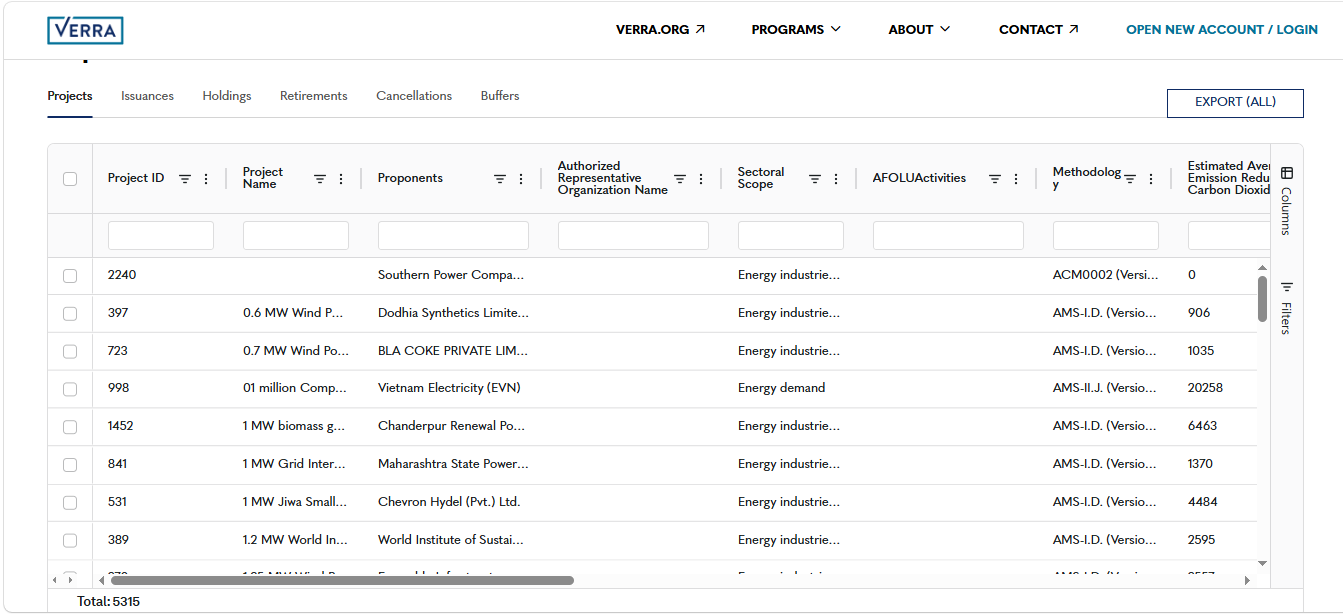
\includegraphics[width=0.85\textwidth]{image/verra_registry.png}
    \caption[Danh sách dự án thuộc chương trình VCS trên Verra Registry]%
    {Danh sách dự án thuộc chương trình VCS trên Verra Registry~\cite{verraregistry}}
    \label{fig:verra}
\end{figure}

National Carbon Credit Registry\index{He thong dang ky@Hệ thống đăng ký (registry)!UNDP National Carbon Registry} của Chương trình phát triển Liên hợp quốc (UNDP) là hệ thống đăng ký quốc gia mã nguồn mở phục vụ Điều~6~\cite{undp2024nationalregistry}. Dữ liệu gốc được ghi trong sổ cái dự án và sổ cái khối tín chỉ, còn PostgreSQL\index{PostgreSQL} chỉ là cơ sở dữ liệu thứ cấp phục vụ truy vấn. Hệ thống chạy trên AWS theo kiến trúc không máy chủ (serverless)\index{Serverless}: hàm Lambda \texttt{national-api} xử lý yêu cầu HTTP, còn hàm \texttt{replicator} được kích hoạt bởi luồng Kinesis để sao chép bản ghi từ sổ cái sang PostgreSQL~\cite{undp2024nationalregistry}. Khi một phần khối tín chỉ (credit block)\index{Khoi tin chi@Khối tín chỉ (Credit Block)} được chuyển nhượng hoặc hủy, hệ thống tách dãy số sê-ri thành hai khối để vẫn truy vết được từng tín chỉ; hệ thống cũng xuất báo cáo theo Định dạng điện tử thỏa thuận (AEF) của Điều~6.2~\cite{undp2024nationalregistry}.

\subsection*{Nền tảng siêu dữ liệu CAD Trust}
\label{subsec:cadtrust}

Climate Action Data Trust (CAD Trust)\index{CAD Trust} không cấp tín chỉ mà là lớp siêu dữ liệu liên kết và chuẩn hóa dữ liệu từ nhiều hệ thống đăng ký như Verra, Gold Standard~\cite{cadtrust2025datamodel}. Mỗi hệ thống đăng ký thành viên chạy một nút của blockchain Chia và tự quản lý dữ liệu của mình; mã băm của mỗi lần cập nhật được ghi lên blockchain để các bên tự đối chiếu và phát hiện dữ liệu bị sửa, còn bản thân dữ liệu nằm trong cơ sở dữ liệu MySQL~\cite{cadtrust2025datamodel}. Mô hình dữ liệu phiên bản 2.0, công bố ngày 23/10/2025, bổ sung các bảng Stakeholders, Methodologies, Validations, Verifications và các bảng AEF cho Điều~6.2 (Bảng~\ref{tab:cadtrust}). Đồ án dùng mô hình CAD Trust V2.0 làm khung cho cơ sở dữ liệu off-chain.

\begin{table}[!htbp]
    \centering
    \caption{Các thực thể dữ liệu chính trong mô hình CAD Trust V2.0}
    \label{tab:cadtrust}
    \small
    \begin{tabularx}{\textwidth}{|L{3.4cm}|Y|}
        \hline
        \HD{Thực thể (bảng)} & \HD{Thuộc tính khóa và mô tả} \\
        \hline
        Project & Mã dự án trên hệ thống đăng ký gốc, chương trình, lĩnh vực, trạng thái; liên kết với Location và Rating \\
        \hline
        Stakeholders & Bảng mới của V2.0: các tổ chức tham gia dự án và vai trò \\
        \hline
        Validations, Verifications & Bảng mới của V2.0: các đợt validation và verification của dự án \\
        \hline
        Issuances & Mỗi bản ghi là một đợt cấp tín chỉ của dự án \\
        \hline
        Units & Khối tín chỉ với dãy số sê-ri, năm vintage\index{Vintage Year}, trạng thái (Issued, Held, Retired); tín chỉ đã hủy có thêm ngày hủy và người thụ hưởng \\
        \hline
        \multicolumn{2}{|l|}{\footnotesize Nguồn: CAD Trust Data Model Version 2.0~\cite{cadtrust2025datamodel}} \\
        \hline
    \end{tabularx}
\end{table}

\subsection*{Khung pháp lý tại Việt Nam}

Văn bản nền tảng là Nghị định 06/2022/NĐ-CP\index{Nghi dinh 06/2022/ND-CP@Nghị định 06/2022/NĐ-CP} về giảm nhẹ phát thải khí nhà kính, đã được sửa đổi bởi các Nghị định 119/2025/NĐ-CP, 83/2026/NĐ-CP, 112/2026/NĐ-CP và 396/2026/NĐ-CP~\cite{vietnam2022nghidinh06}. Nghị định quy định kiểm kê khí nhà kính, phân bổ hạn ngạch\index{Han ngach phat thai@Hạn ngạch phát thải} cho các cơ sở phát thải lớn và cơ chế trao đổi, bù trừ tín chỉ; theo Điều~19 được thay thế bởi Nghị định 119/2025/NĐ-CP, cơ sở được dùng tín chỉ để bù trừ không quá 30\% hạn ngạch được phân bổ~\cite{vietnam2025nghidinh119}. Vì vậy, hệ thống tại Việt Nam phải phân biệt tín chỉ tự nguyện (như VCU) với hạn ngạch và tín chỉ của thị trường trong nước. Hạ tầng của thị trường gồm Hệ thống đăng ký quốc gia\index{He thong dang ky quoc gia@Hệ thống đăng ký quốc gia} theo Thông tư 11/2026/TT-BNNMT~\cite{vietnam2026thongtu11} và sàn giao dịch theo Nghị định 29/2026/NĐ-CP~\cite{vietnam2026nghidinh29}; Nghị định 396/2026/NĐ-CP, có hiệu lực từ ngày 12/12/2026, phân cấp việc cấp tín chỉ theo cơ chế trong nước cho Chủ tịch Ủy ban nhân dân cấp tỉnh~\cite{vietnam2026nghidinh396}. Ngoài thị trường trong nước, năm 2020 Việt Nam ký Thỏa thuận chi trả giảm phát thải (ERPA)\index{ERPA} với Ngân hàng Thế giới, theo đó được chi trả tới 51,5 triệu USD cho 10,3 triệu tấn CO$_2$ giảm phát thải từ rừng tại sáu tỉnh Bắc Trung Bộ đến năm 2025~\cite{worldbank2020erpa}.

% ------------------------------------------------------------
\section{Khảo sát sơ bộ hệ thống}
\label{sec:khaosatsobo}
% Thời gian khảo sát: tháng 9–11/2026 (nguồn truy cập ngày 28/9, 20/10 và 04/11/2026).

\FloatBarrier
\subsection*{Mục tiêu, phạm vi và phương pháp khảo sát}
\label{subsec:ks-gioithieu}

Khảo sát nhằm xác định các bên liên quan, quy trình, dữ liệu và công cụ của các hệ thống đang vận hành, đánh giá ưu, nhược điểm của chúng và rút ra nhu cầu cho hệ thống mới. Phạm vi tập trung vào giai đoạn sau khi tín chỉ được cấp (đăng ký, định danh, chuyển quyền sở hữu, giao dịch, hủy); khâu MRV tại thực địa chỉ được xem ở mức đầu vào. Các hệ thống được khảo sát gồm hạ tầng trong nước (Hệ thống đăng ký quốc gia, hệ thống của sàn giao dịch) và các hệ thống quốc tế (Verra Registry, UNDP National Carbon Registry, CAD Trust, Toucan Protocol).

Do chưa tiếp cận được người dùng thực tế, khảo sát kết hợp hai phương pháp. Nghiên cứu tài liệu dựa trên văn bản pháp luật (nguồn chính thức về quy trình và trách nhiệm của từng bên), tài liệu kỹ thuật của các hệ thống quốc tế và các bài báo khoa học~\cite{kim2020blockchain,sipthorpe2022blockchain,vaccargiu2026blockchain}. Quan sát gồm truy cập trang công khai của các hệ thống không cần đăng nhập, đọc quy trình nội bộ mà cơ quan quản lý đã ban hành và thu thập số liệu vận hành đã công bố. Vì vậy, kết quả chủ yếu phản ánh quy trình theo quy định, chưa phản ánh đầy đủ khó khăn thực tế của người dùng.
% [VIẾT SAU - PHỎNG VẤN] Phỏng vấn 1–2 chuyên gia (đơn vị tư vấn các-bon, công ty chứng khoán thành viên),
% mỗi buổi 20–30 phút. Câu hỏi gợi ý: Q1 (VĐ-1) kiểm tra trùng đăng ký Verra/Gold Standard thế nào;
% Q2 (VĐ-2) chứng minh tín chỉ đã hủy bằng giấy tờ gì; Q3 (VĐ-3) báo cáo thẩm định được lưu, ký thế nào;
% Q4 (VĐ-4) đối soát giữa Hệ thống đăng ký quốc gia, HNX, VSDC tốn bao nhiêu nhân lực; Q5 (VĐ-5) vì sao
% thanh khoản thấp; Q6 dữ liệu nào được phép công khai. Kết quả: bổ sung phương pháp phỏng vấn vào đoạn trên
% và thêm ý kiến chuyên gia vào phần đánh giá.

\FloatBarrier
\subsection*{Hiện trạng hệ thống trong nước}
\label{subsec:ks-tongquan}
\label{subsec:ks-hientrang}

Thị trường tín chỉ các-bon không do một đơn vị duy nhất vận hành (\autoref{fig:mohinhtochuc}). Bộ Nông nghiệp và Môi trường là cơ quan duy nhất cấp mã trong nước và số sê-ri cho hạn ngạch, tín chỉ; Cục Biến đổi khí hậu vận hành Hệ thống đăng ký quốc gia, nơi lưu dữ liệu gốc về chủ sở hữu, số lượng, mã, số sê-ri, trạng thái và lịch sử giao dịch~\cite{vietnam2026thongtu11}. Sở Giao dịch Chứng khoán Hà Nội (HNX)\index{HNX} tổ chức giao dịch, Tổng công ty Lưu ký và Bù trừ Chứng khoán Việt Nam (VSDC)\index{VSDC} phụ trách lưu ký, chuyển quyền sở hữu và thanh toán~\cite{vietnam2026nghidinh29}. Mỗi tổ chức chỉ được cấp một tài khoản đăng ký, gắn với mã số thuế~\cite{vietnam2026thongtu11}. Bảng~\ref{tab:ks-tacnhan} tổng hợp các bên tham gia; Bảng~\ref{tab:ks-hethong} liệt kê các hệ thống được khảo sát.

\HinhMoHinhToChuc

\begin{table}[!htbp]
    \centering
    \caption{Các đối tượng tham gia vòng đời tín chỉ các-bon}
    \label{tab:ks-tacnhan}
    \label{tab:ks-doituong}
    \small
    \begin{tabularx}{\textwidth}{|L{3.3cm}|Y|L{3.8cm}|}
        \hline
        \HD{Đối tượng} & \HD{Vai trò} & \HD{Hệ thống sử dụng} \\
        \hline
        Chủ dự án & Lập hồ sơ, giám sát, nhận và sở hữu tín chỉ & Hệ thống đăng ký quốc gia; Verra Registry \\
        \hline
        Đơn vị thẩm định độc lập (VVB) & Thẩm định hồ sơ và kết quả giảm phát thải theo ISO 14064-3 & Nộp báo cáo cho chương trình hoặc cơ quan cấp \\
        \hline
        Cơ quan quản lý (cấp bộ, cấp tỉnh) & Quyết định cấp tín chỉ, cấp mã và số sê-ri, quản lý tài khoản, đối soát, công bố thông tin & Hệ thống đăng ký quốc gia \\
        \hline
        Cơ sở được phân bổ hạn ngạch & Mua tín chỉ, bù trừ phát thải, nộp trả hạn ngạch & Hệ thống đăng ký quốc gia, tài khoản lưu ký và giao dịch \\
        \hline
        HNX, VSDC, ngân hàng & Tổ chức giao dịch, lưu ký, thanh toán, báo cáo & Hệ thống giao dịch, lưu ký và thanh toán \\
        \hline
        Người dùng công khai & Tra cứu dự án, tín chỉ đã cấp và đã hủy & Thông tin công bố; trang tra cứu Verra Registry \\
        \hline
    \end{tabularx}
\end{table}

\begin{table}[!htbp]
    \centering
    \caption{Các hệ thống đang sử dụng trong vòng đời tín chỉ các-bon}
    \label{tab:ks-hethong}
    \small
    \begin{tabularx}{\textwidth}{|L{3.2cm}|L{2.6cm}|Y|L{2.6cm}|}
        \hline
        \HD{Hệ thống} & \HD{Đơn vị vận hành} & \HD{Chức năng chính} & \HD{Nền tảng} \\
        \hline
        Hệ thống đăng ký quốc gia~\cite{vietnam2026thongtu11} & Cục Biến đổi khí hậu & Tài khoản, mã trong nước, số sê-ri, ký gửi, bù trừ, hủy & Tập trung, xác thực qua Cổng dịch vụ công quốc gia \\
        \hline
        Hệ thống giao dịch, lưu ký~\cite{vietnam2026nghidinh29} & HNX, VSDC & Khớp lệnh, lưu ký, chuyển quyền sở hữu, thanh toán & Tập trung \\
        \hline
        Verra Registry~\cite{verra2024vcs} & Verra & Đăng ký dự án, cấp VCU có số sê-ri, hủy, tra cứu & Tập trung, web \\
        \hline
        UNDP National Carbon Registry~\cite{undp2024nationalregistry} & Từng quốc gia & Đăng ký quốc gia mã nguồn mở, báo cáo AEF & Sổ cái, PostgreSQL trên AWS \\
        \hline
        CAD Trust~\cite{cadtrust2025datamodel} & CAD Trust & Siêu dữ liệu liên thông các hệ thống đăng ký & Blockchain Chia, MySQL \\
        \hline
        Toucan Protocol~\cite{toucan2025docs} & Toucan & Token hóa tín chỉ, pool ERC-20, hủy on-chain & Polygon, Celo \\
        \hline
    \end{tabularx}
\end{table}

Theo Thông tư 11/2026/TT-BNNMT, vòng đời một tín chỉ trên hệ thống trong nước gồm ba nhóm quy trình~\cite{vietnam2026thongtu11,vietnam2026nghidinh29}:
\begin{itemize}
    \item Đăng ký: sau khi cơ quan có thẩm quyền quyết định cấp, trong 05 ngày làm việc Bộ đăng ký tín chỉ (chương trình, cơ chế, số lượng, mã trong nước, chủ sở hữu, số sê-ri) và gửi mã trong nước cho HNX, VSDC.
    \item Ký gửi và giao dịch: chủ tài khoản muốn giao dịch phải ký gửi tín chỉ sang hệ thống lưu ký qua bốn bước:
    \begin{enumerate}
        \item chủ tài khoản thông báo số lượng cần ký gửi; hệ thống chuyển số lượng này từ tiểu khoản Đăng ký chung sang tiểu khoản Chờ ký gửi, hoặc từ chối nếu số dư không đủ;
        \item cuối mỗi ngày làm việc, Bộ tổng hợp danh sách đề nghị ký gửi và gửi cho VSDC;
        \item trong 01 ngày làm việc, VSDC xác nhận hoặc từ chối; khi được xác nhận, số lượng được chuyển sang tiểu khoản Số dư giao dịch;
        \item lệnh được khớp trên hệ thống của HNX; VSDC chuyển quyền sở hữu và thanh toán qua ngân hàng thanh toán.
    \end{enumerate}
    Cuối mỗi ngày, VSDC gửi báo cáo kết quả thanh toán và số dư ký gửi để Bộ đối soát với dữ liệu trên Hệ thống đăng ký quốc gia (Điều~23).
    \item Bù trừ và hủy: tín chỉ bị hủy khi dùng để bù trừ, khi chủ tài khoản hủy tự nguyện (xử lý trong 02 ngày làm việc) hoặc khi bị thu hồi; việc hủy gồm cả số lượng và số sê-ri, và mã trong nước đã hủy không được cấp lại.
\end{itemize}

Dữ liệu cốt lõi là mã trong nước\index{Ma trong nuoc@Mã trong nước} và số sê-ri. Mã của hạn ngạch có dạng VN[năm], ví dụ VN2025; mã của tín chỉ gồm 9 ký tự (mã cơ chế, mã dự án, năm xác nhận); số sê-ri nối mã trong nước với 10 chữ số thứ tự, nên mỗi tấn CO$_2$e có một số sê-ri riêng~\cite{vietnam2026thongtu11}. Mỗi tài khoản có 8 tiểu khoản\index{Tieu khoan@Tiểu khoản} theo Điều~7 Thông tư 11/2026/TT-BNNMT, tương ứng với các trạng thái mà một đơn vị hạn ngạch hoặc tín chỉ có thể đi qua (Bảng~\ref{tab:ks-tieukhoan}); khi đổi trạng thái, số lượng được chuyển giữa các tiểu khoản, và các nghiệp vụ ký gửi, chuyển quyền sở hữu, chuyển giao, vay mượn chỉ thực hiện được với số lượng đang ở tiểu khoản Đăng ký chung~\cite{vietnam2026thongtu11}.

\begin{table}[!htbp]
    \centering
    \caption{Các tiểu khoản của tài khoản đăng ký theo Thông tư 11/2026/TT-BNNMT}
    \label{tab:ks-tieukhoan}
    \begin{tabularx}{\textwidth}{|L{3.2cm}|Y|}
        \hline
        \HD{Tiểu khoản} & \HD{Nội dung ghi nhận} \\
        \hline
        Đăng ký chung & Hạn ngạch, tín chỉ thuộc sở hữu hợp pháp của chủ tài khoản, chưa đưa vào giao dịch hay nghiệp vụ khác \\
        \hline
        Chờ ký gửi & Hạn ngạch, tín chỉ đã đề nghị ký gửi, đang chờ VSDC xác nhận \\
        \hline
        Số dư giao dịch & Hạn ngạch, tín chỉ đã ký gửi tại VSDC \\
        \hline
        Bù trừ & Tín chỉ được dùng để bù trừ phát thải \\
        \hline
        Nộp trả & Hạn ngạch được chủ tài khoản nộp trả \\
        \hline
        Chuyển giao & Hạn ngạch chuyển từ giai đoạn hiện tại sang giai đoạn kế tiếp \\
        \hline
        Vay mượn & Hạn ngạch của giai đoạn kế tiếp được vay để dùng cho giai đoạn hiện tại \\
        \hline
        Phong tỏa & Hạn ngạch, tín chỉ bị phong tỏa theo yêu cầu của cơ quan có thẩm quyền \\
        \hline
        \multicolumn{2}{|l|}{\footnotesize Nguồn: Điều~7 Thông tư 11/2026/TT-BNNMT~\cite{vietnam2026thongtu11}} \\
        \hline
    \end{tabularx}
\end{table}

Về công bố thông tin, Bộ công bố hằng tháng (chậm nhất ngày 20 tháng sau) danh sách dự án đã đăng ký và tổng số lượng đăng ký mới, hủy đăng ký, đồng thời công bố trong vòng 72 giờ việc cấp, hủy mã trong nước và số sê-ri; thông tin truy cập và thông tin giao dịch của các tổ chức phải được bảo mật~\cite{vietnam2026thongtu11}. Các công cụ hỗ trợ gồm xác thực qua Cổng dịch vụ công quốc gia, cơ chế một người tạo và một người khác duyệt mỗi giao dịch, kết nối với HNX, VSDC qua kênh riêng hoặc API mã hóa, và công bố thông tin định kỳ theo tháng, năm~\cite{vietnam2026thongtu11}.

\FloatBarrier
\subsection*{Quan sát các hệ thống thực tế}
\label{subsec:ks-quansat}

Để kiểm tra các nhận định rút ra từ văn bản, đồ án truy cập trang công khai của một số hệ thống ngày 04/11/2026. Bảng~\ref{tab:ks-quansat} tóm tắt kết quả; \autoref{fig:ks-dvc-taikhoan} đến \autoref{fig:ks-toucan} là ảnh chụp màn hình các trang được quan sát.

\begin{table}[!htbp]
    \centering
    \caption{Kết quả quan sát các hệ thống thực tế}
    \label{tab:ks-quansat}
    \label{tab:ks-quansat-qt}
    \small
    \begin{tabularx}{\textwidth}{|L{3.0cm}|Y|}
        \hline
        \HD{Hệ thống} & \HD{Kết quả ghi nhận} \\
        \hline
        Thủ tục đăng ký tài khoản (mã 1.014129) & Hồ sơ nộp trực tiếp, trực tuyến hoặc qua bưu chính; thời hạn 05 ngày làm việc; hồ sơ qua chuyên viên, lãnh đạo phòng, lãnh đạo Cục và lãnh đạo Bộ duyệt~\cite{mae2026tthc1014129,mae2025qd2935} \\
        \hline
        Thủ tục cấp tín chỉ trong nước (mã 1.014133) & Trang thủ tục vẫn hiển thị quy trình cũ: bộ quản lý lĩnh vực quyết định, tổng 06 ngày làm việc và 30 ngày, có nhánh bổ sung hồ sơ~\cite{mae2026tthc1014133}; từ ngày 12/12/2026, Chủ tịch Ủy ban nhân dân cấp tỉnh quyết định trong tối đa 26 ngày làm việc~\cite{vietnam2026nghidinh396} \\
        \hline
        Sàn giao dịch các-bon (HNX) & VN2025 là mã duy nhất (511.473.846 tấn CO$_2$e hạn ngạch, giao dịch từ 29/6/2026 đến 24/12/2027)~\cite{hnx2026vn2025,hnx2026danhmuchanngach}; khối lượng giao dịch theo tháng rất nhỏ, chưa có tín chỉ nào được giao dịch~\cite{hnx2026sanphamcacbon}; trang thống kê giao dịch chưa công bố số liệu tổng hợp~\cite{hnx2026ketquagd} \\
        \hline
        Verra Registry & Ai cũng tra cứu được, nhưng phát hành, chuyển nhượng, hủy cần tài khoản; báo cáo Retirements công khai từng lô với ngày hủy, dự án, vintage, số sê-ri; người thụ hưởng và lý do hủy có thể ẩn~\cite{verraregistry,verra2020registryv2} \\
        % [VIẾT SAU - SỐ LIỆU] Lọc Retirement Date = 04/11/2026, ghi tổng số lô được hủy trong ngày.
        \hline
        CAD Trust & Dashboard công khai chỉ có số liệu tổng hợp theo khu vực, quốc gia; không tìm thấy trang chi tiết dự án khi không đăng nhập~\cite{cadtrust2026dashboard} \\
        % [VIẾT SAU - ẢNH CHỤP] Chọn Southeast Asia -> Viet Nam trên dashboard, ghi số dự án và nội dung ô Registry.
        \hline
        Toucan Protocol & Trang dự án Wakefield Biochar Facility 2 giữ mã dự án PUR-244045 của tiêu chuẩn gốc Puro và cho biết tín chỉ đã nằm trong pool CHAR~\cite{toucan2026wakefield} \\
        \hline
    \end{tabularx}
\end{table}

\begin{figure}[!htbp]
    \centering
    \begin{subfigure}{\textwidth}
        \centering
        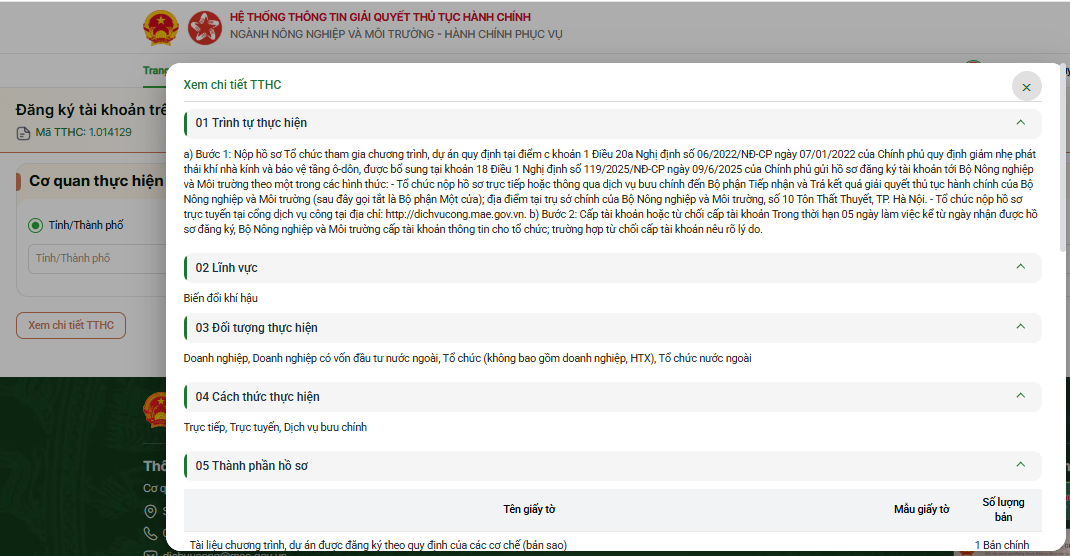
\includegraphics[width=0.8\textwidth]{image/dvc_1014129_trinh_tu.png}
        \caption{Trình tự thực hiện}
    \end{subfigure}

    \vspace{0.3cm}
    \begin{subfigure}{\textwidth}
        \centering
        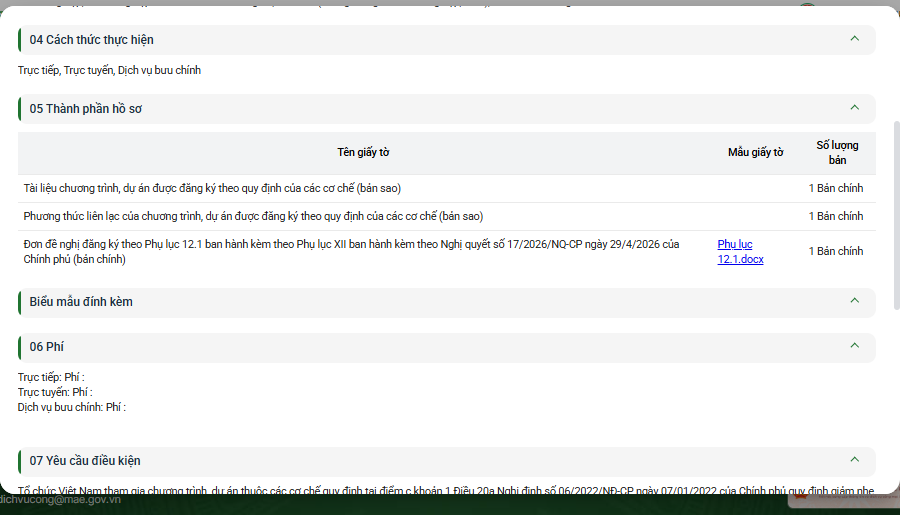
\includegraphics[width=0.68\textwidth]{image/dvc_1014129_ho_so.png}
        \caption{Thành phần hồ sơ}
    \end{subfigure}

    \vspace{0.3cm}
    \begin{subfigure}{\textwidth}
        \centering
        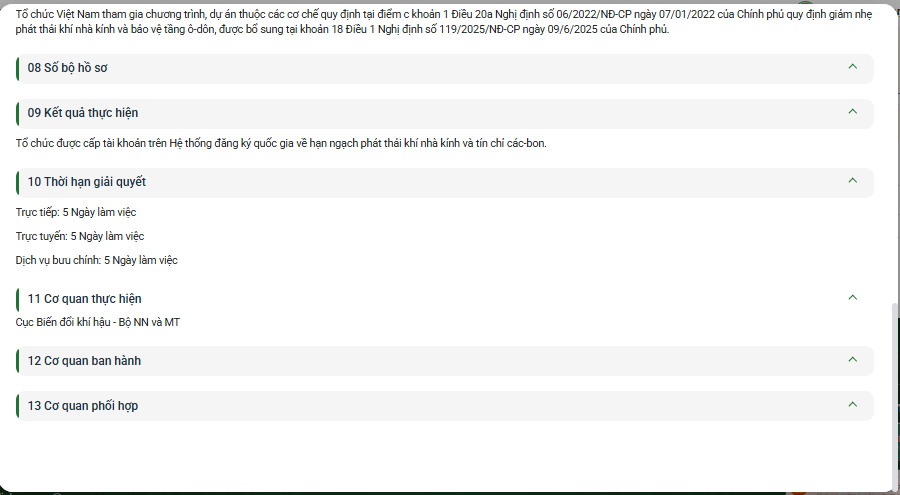
\includegraphics[width=0.68\textwidth]{image/dvc_1014129_thoi_han.png}
        \caption{Kết quả, thời hạn giải quyết và cơ quan thực hiện}
    \end{subfigure}
    \caption[Trang thủ tục đăng ký tài khoản trên Hệ thống đăng ký quốc gia]%
    {Trang thủ tục mã 1.014129 về đăng ký tài khoản trên Hệ thống đăng ký quốc gia (truy cập ngày 04/11/2026)~\cite{mae2026tthc1014129}}
    \label{fig:ks-dvc-taikhoan}
\end{figure}

\begin{figure}[!htbp]
    \centering
    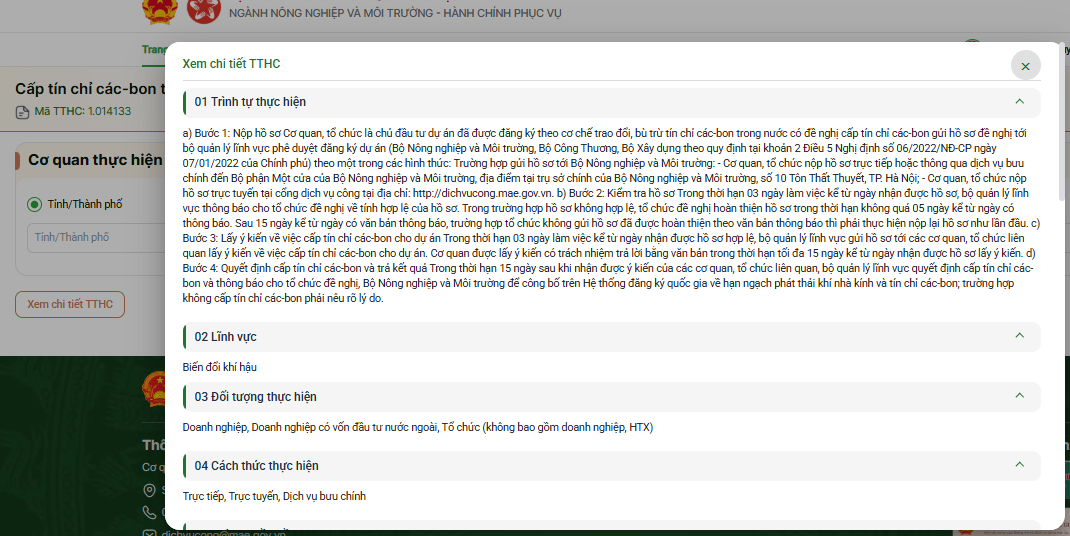
\includegraphics[width=0.85\textwidth]{image/dvc_1014133_trinh_tu.png}
    \caption[Trang thủ tục cấp tín chỉ các-bon theo cơ chế trong nước]%
    {Trang thủ tục mã 1.014133 về cấp tín chỉ các-bon theo cơ chế trong nước, trình tự bốn bước trước Nghị định 396/2026/NĐ-CP (truy cập ngày 04/11/2026)~\cite{mae2026tthc1014133}}
    \label{fig:ks-dvc-tinchi}
\end{figure}

\begin{figure}[!htbp]
    \centering
    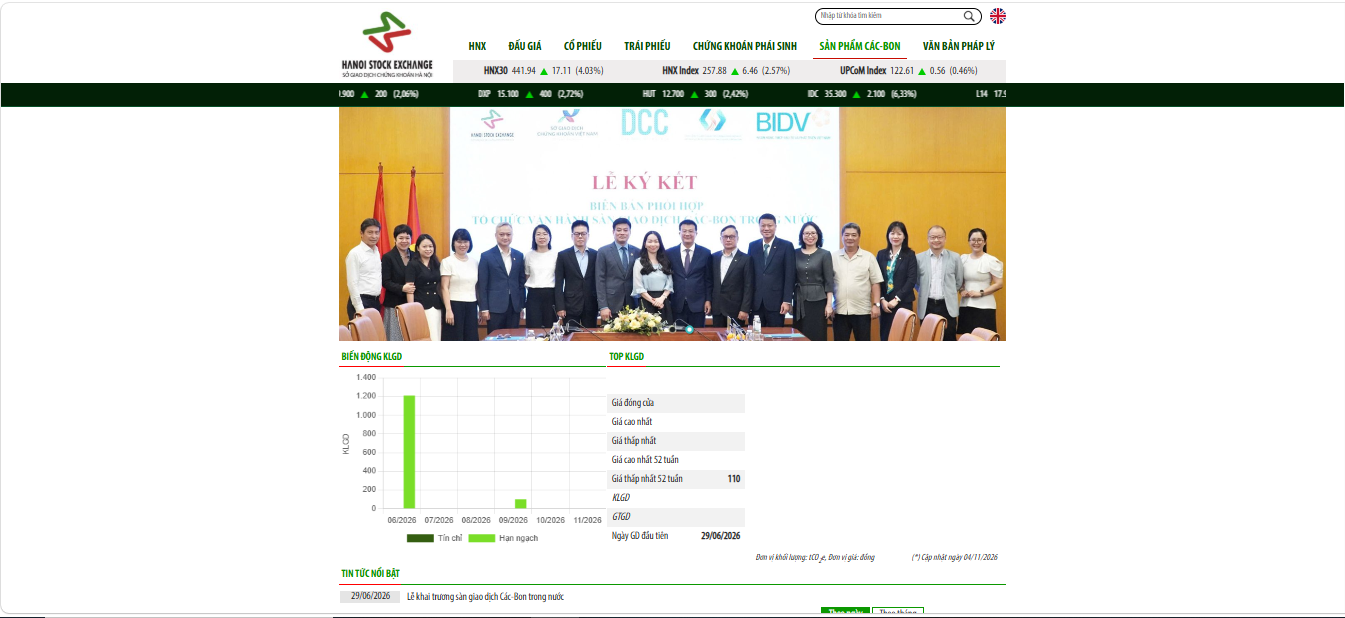
\includegraphics[width=0.9\textwidth]{image/hnx_san_cacbon.png}
    \caption[Trang sản phẩm các-bon trên website của HNX]%
    {Trang sản phẩm các-bon của HNX: khối lượng giao dịch theo tháng và thông tin mã VN2025 (truy cập ngày 04/11/2026)~\cite{hnx2026sanphamcacbon}}
    \label{fig:ks-hnx}
\end{figure}

\begin{figure}[!htbp]
    \centering
    \begin{subfigure}{\textwidth}
        \centering
        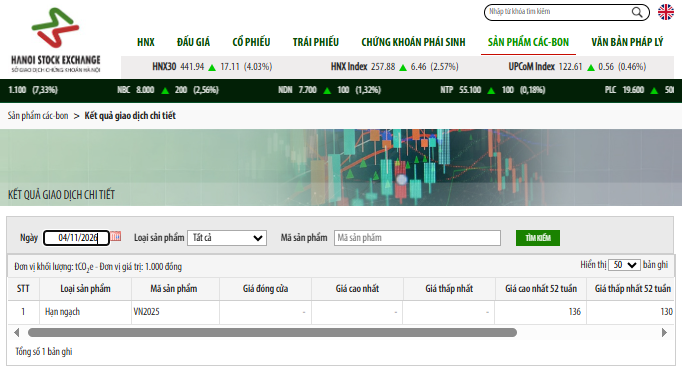
\includegraphics[width=0.75\textwidth]{image/hnx_ket_qua_giao_dich.png}
        \caption{Kết quả giao dịch chi tiết ngày 04/11/2026~\cite{hnx2026ketquagd}}
    \end{subfigure}

    \vspace{0.3cm}
    \begin{subfigure}{\textwidth}
        \centering
        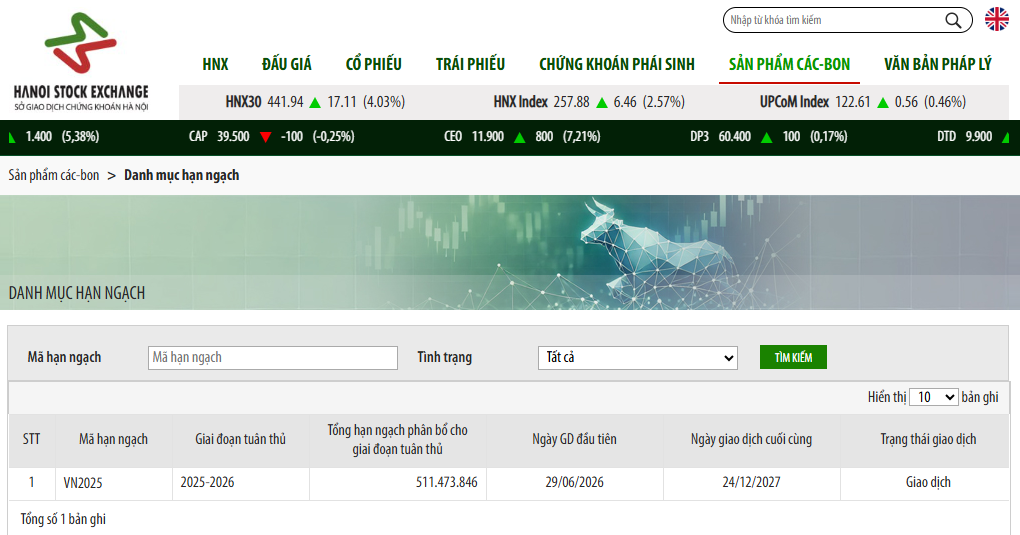
\includegraphics[width=0.85\textwidth]{image/hnx_danh_muc_han_ngach.png}
        \caption{Danh mục hạn ngạch~\cite{hnx2026danhmuchanngach}}
    \end{subfigure}
    \caption[Kết quả giao dịch và danh mục hạn ngạch trên website của HNX]%
    {Kết quả giao dịch và danh mục hạn ngạch trên trang sản phẩm các-bon của HNX (truy cập ngày 04/11/2026)}
    \label{fig:ks-hnx-chitiet}
\end{figure}

\begin{figure}[!htbp]
    \centering
    \begin{subfigure}{\textwidth}
        \centering
        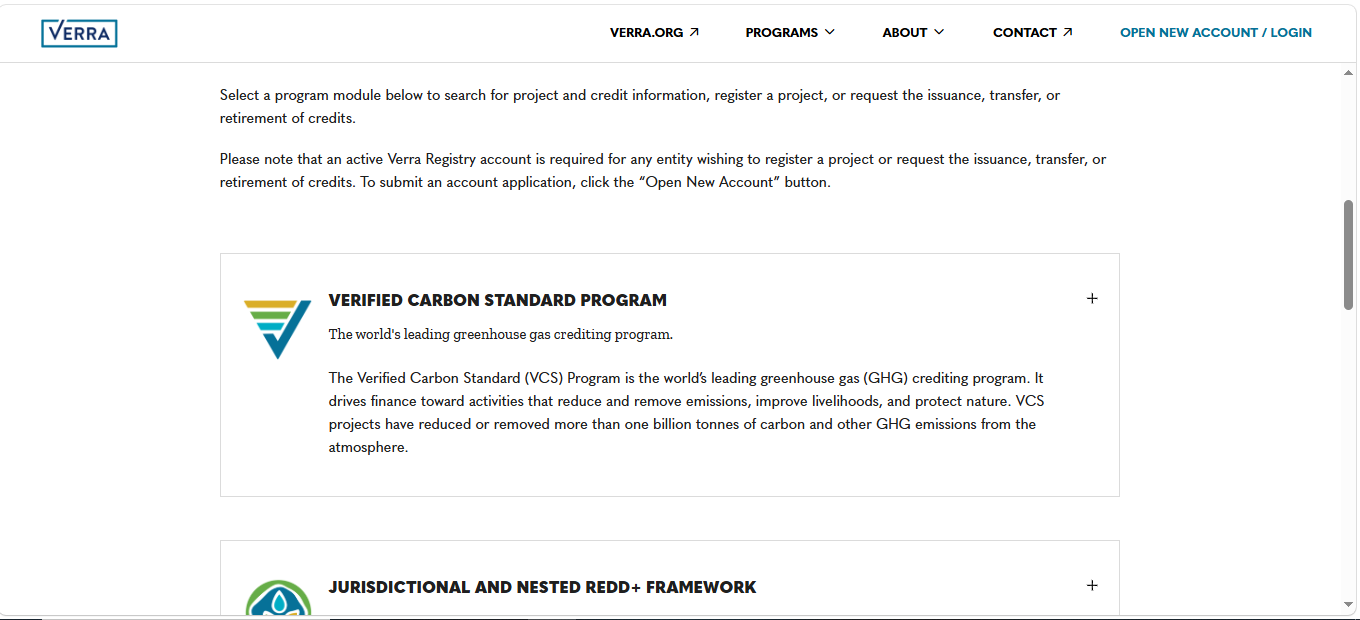
\includegraphics[width=0.85\textwidth]{image/verra_registry_home.png}
        \caption{Trang chủ: tra cứu theo chương trình là công khai, còn đăng ký, phát hành, chuyển nhượng và hủy tín chỉ yêu cầu tài khoản~\cite{verraregistry}}
    \end{subfigure}

    \vspace{0.3cm}
    \begin{subfigure}{\textwidth}
        \centering
        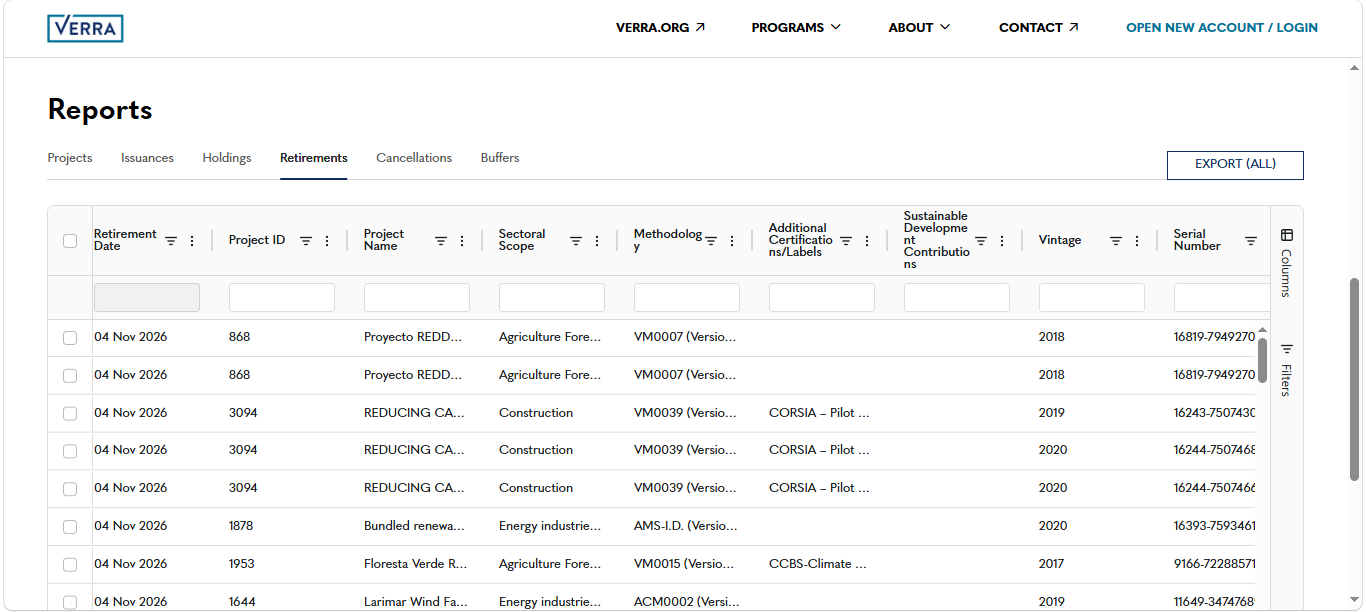
\includegraphics[width=0.85\textwidth]{image/verra_retirements.png}
        \caption{Báo cáo Retirements: mỗi dòng là một lô tín chỉ đã hủy, có ngày hủy, dự án, vintage và số sê-ri~\cite{verraregistry}}
    \end{subfigure}
    \caption[Trang công khai của Verra Registry]%
    {Trang công khai của Verra Registry (truy cập ngày 04/11/2026)}
    \label{fig:ks-verra}
\end{figure}

% [VIẾT SAU - ẢNH CHỤP] Thay bằng ảnh dashboard của Việt Nam (Southeast Asia -> Viet Nam) và sửa chú thích.
\begin{figure}[!htbp]
    \centering
    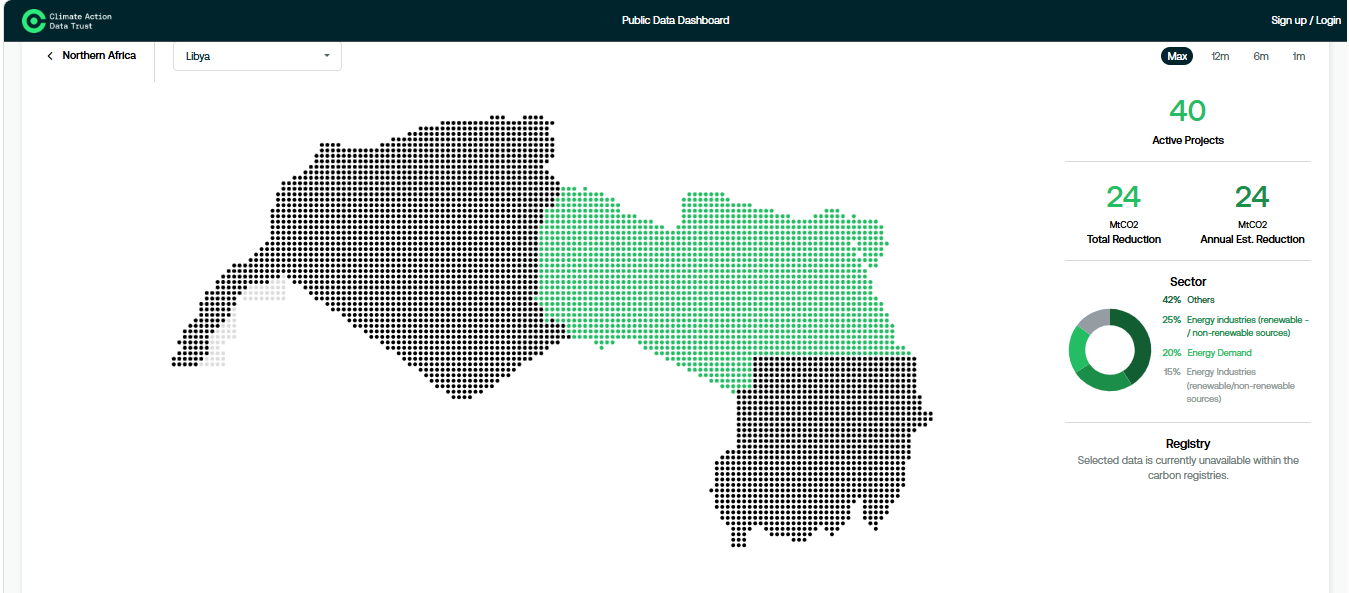
\includegraphics[width=0.85\textwidth]{image/cadtrust_dashboard.png}
    \caption[Public Data Dashboard của CAD Trust]%
    {Public Data Dashboard của CAD Trust: số liệu tổng hợp của một quốc gia gồm số dự án, lượng giảm phát thải và cơ cấu theo lĩnh vực (truy cập ngày 04/11/2026)~\cite{cadtrust2026dashboard}}
    \label{fig:ks-cadtrust}
\end{figure}

\begin{figure}[!htbp]
    \centering
    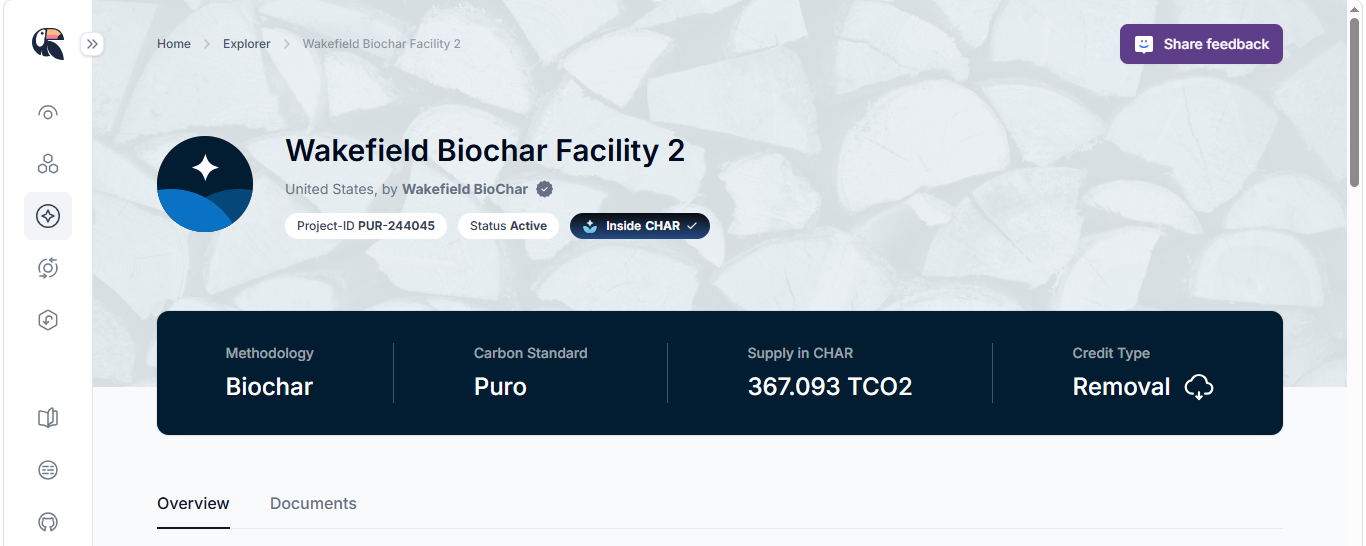
\includegraphics[width=0.85\textwidth]{image/toucan_project.png}
    \caption[Trang một dự án trên ứng dụng Toucan]%
    {Trang dự án Wakefield Biochar Facility 2 trên ứng dụng Toucan: mã dự án, tiêu chuẩn gốc, phương pháp luận, loại tín chỉ và pool chứa token (truy cập ngày 04/11/2026)~\cite{toucan2026wakefield}}
    \label{fig:ks-toucan}
\end{figure}

Từ kết quả quan sát rút ra bốn nhận xét.

Thứ nhất, nghiệp vụ trong nước đi qua nhiều cấp phê duyệt và nhiều hệ thống: một giao dịch cần dữ liệu ở Hệ thống đăng ký quốc gia, hệ thống giao dịch của HNX, hệ thống lưu ký của VSDC và tài khoản tại công ty chứng khoán. Mỗi bước của thủ tục cấp tín chỉ có thời hạn riêng và có nhánh quay lại khi hồ sơ phải bổ sung. Theo Nghị định 396/2026/NĐ-CP, từ ngày 12/12/2026 việc cấp tín chỉ trong nước mất tối đa 26 ngày làm việc, so với khoảng 27 đến 28 ngày làm việc của quy trình cũ~\cite{vietnam2026nghidinh396}. Thay đổi lớn hơn là thẩm quyền được phân cấp xuống cấp tỉnh: tín chỉ sẽ được cấp ở nhiều địa phương nhưng vẫn phải ghi nhận thống nhất trên Hệ thống đăng ký quốc gia, nên hệ thống mới cần cho phép nhiều tài khoản cùng có quyền phát hành (NC-09).

Thứ hai, thị trường chưa có thanh khoản: đến ngày 04/11/2026 hàng hóa duy nhất là hạn ngạch, nên chưa có dữ liệu thực tế về giao dịch tín chỉ trong nước để hệ thống của đồ án sử dụng.

Thứ ba, Verra Registry tách rõ phần tra cứu công khai và phần nghiệp vụ cần tài khoản; báo cáo hủy tín chỉ công khai tới từng lô và số sê-ri nhưng thông tin người thụ hưởng có thể được ẩn, cho thấy yêu cầu minh bạch luôn đi kèm giới hạn về riêng tư.

Thứ tư, các hệ thống tổng hợp dữ liệu hoặc token hóa tín chỉ đều dựa vào hệ thống đăng ký gốc: CAD Trust chỉ hiển thị được số liệu mà các hệ thống đăng ký cung cấp, còn dự án được quan sát trên Toucan là tín chỉ do Puro cấp và vẫn giữ mã dự án của Puro. Vì vậy, mỗi bản ghi tín chỉ trên blockchain cần giữ liên kết tới mã dự án và số sê-ri do hệ thống đăng ký gốc cấp.

\FloatBarrier
\subsection*{Đánh giá hệ thống hiện tại}
\label{subsec:ks-danhgia}

Hệ thống trong nước có cơ sở pháp lý rõ ràng, dữ liệu gốc thống nhất, số sê-ri tới từng tấn CO$_2$e, mô hình tám tiểu khoản chặt chẽ và định danh pháp lý qua Cổng dịch vụ công quốc gia; các hệ thống quốc tế đóng góp các ý tưởng như tra cứu công khai (Verra), mã nguồn mở và tách khối sê-ri (UNDP), mô hình dữ liệu chung (CAD Trust) và hủy tín chỉ công khai trên blockchain (Toucan). Bảng~\ref{tab:ks-uunhuoc} tóm tắt ưu, nhược điểm của từng hệ thống.

\begin{table}[!htbp]
    \centering
    \caption{Ưu điểm và nhược điểm của các hệ thống được khảo sát}
    \label{tab:ks-uunhuoc}
    \small
    \begin{tabularx}{\textwidth}{|L{2.8cm}|Y|Y|}
        \hline
        \HD{Hệ thống} & \HD{Ưu điểm} & \HD{Nhược điểm} \\
        \hline
        Hệ thống trong nước & Pháp lý rõ ràng; dữ liệu gốc thống nhất; số sê-ri tới từng đơn vị; xác thực định danh điện tử & Đang thí điểm; ba hệ thống phải đối soát cuối ngày; công khai chủ yếu ở dạng tổng hợp; bên ngoài không tự kiểm chứng được lịch sử tín chỉ \\
        \hline
        Verra Registry & Quy mô lớn; số sê-ri duy nhất; tra cứu công khai & Tập trung; chưa có API công khai; không liên thông với hệ thống khác \\
        \hline
        UNDP National Carbon Registry & Mã nguồn mở; hỗ trợ Điều~6 và AEF; tách dãy sê-ri & Mỗi quốc gia tự vận hành hạ tầng; sổ cái do một bên quản lý \\
        \hline
        CAD Trust & Liên thông nhiều hệ thống; mô hình dữ liệu chung; mã băm trên blockchain & Không ghi quyền sở hữu, không giao dịch; mã băm chứng minh dữ liệu không bị sửa, không chứng minh dữ liệu đúng \\
        \hline
        Toucan Protocol & Hủy tín chỉ và chứng nhận hủy công khai on-chain & Phụ thuộc hệ thống đăng ký gốc; Verra đã cấm token hóa tín chỉ đã hủy~\cite{verra2022crypto}; pool làm mất thông tin riêng của dự án \\
        \hline
    \end{tabularx}
\end{table}

Đối với hệ thống trong nước, các nhược điểm chính là:
\begin{itemize}
    \item Tính toàn vẹn dựa vào niềm tin vào đơn vị vận hành: các ràng buộc như mã trong nước không được cấp lại sau khi hủy hay không hủy quá số dư được bảo đảm bởi phần mềm và quy trình của cơ quan quản lý; bên mua hoặc tổ chức bên ngoài không có công cụ để tự kiểm chứng rằng một số sê-ri chưa từng được cấp cho người khác hoặc chưa từng bị hủy.
    \item Dữ liệu phân tán giữa nhiều hệ thống: cùng một lượng tín chỉ được ghi ở Hệ thống đăng ký quốc gia và ở hệ thống lưu ký của VSDC, nên phải đối soát cuối mỗi ngày và có quy trình xử lý sai lệch~\cite{vietnam2026thongtu11}.
    \item Độ trễ trong nghiệp vụ: ký gửi chờ tổng hợp cuối ngày và chờ VSDC xác nhận trong 01 ngày làm việc; hủy tự nguyện được xử lý trong 02 ngày làm việc~\cite{vietnam2026thongtu11}.
    \item Mức độ công khai hạn chế: dữ liệu công bố chủ yếu là số liệu tổng hợp theo tháng, năm, còn thông tin giao dịch được bảo mật; điều này phù hợp yêu cầu bảo mật nhưng khiến bên thứ ba khó truy vết lịch sử của một tín chỉ cụ thể, và tại thời điểm khảo sát chưa có tài liệu API công khai cho bên thứ ba.
    \item Khâu MRV chưa được số hóa đồng bộ: hồ sơ dự án, báo cáo giám sát và báo cáo thẩm định vẫn là các tệp được nộp qua từng bước, chưa gắn với tín chỉ được cấp bằng một dấu vết kiểm chứng được~\cite{mae2026tthc1014133}.
\end{itemize}

Từ các nhược điểm trên, đồ án xác định năm vấn đề làm cơ sở cho nhu cầu của hệ thống mới:
\begin{enumerate}[label=VĐ-\arabic*., leftmargin=1.6cm]
    \item Rủi ro phát hành kép giữa các hệ thống: hệ thống trong nước và các chương trình quốc tế dùng không gian định danh khác nhau; nếu không liên thông dữ liệu, một dự án có thể được đăng ký ở nhiều nơi~\cite{schneider2019double}.
    \item Bên mua khó chứng minh tín chỉ đã được hủy: bằng chứng hiện nay chủ yếu là thông báo xác nhận do cơ quan quản lý gửi cho chủ tài khoản, bên thứ ba không tự kiểm tra được.
    \item Hồ sơ MRV và thẩm định không gắn chặt với tín chỉ: không có cơ chế kỹ thuật bảo đảm hồ sơ không bị sửa sau khi cấp hoặc không bị dùng lại cho lần cấp khác.
    \item Chi phí đối soát giữa nhiều cơ sở dữ liệu: cùng một lượng tín chỉ được ghi ở ba hệ thống, các bên phải đối soát cuối mỗi ngày và duy trì quy trình xử lý sai lệch~\cite{vietnam2026thongtu11}.
    \item Thị trường còn ở giai đoạn đầu và quy định đang thay đổi (ví dụ phân cấp cho cấp tỉnh theo Nghị định 396/2026/NĐ-CP~\cite{vietnam2026nghidinh396}), nên hệ thống mới cần linh hoạt về phân quyền.
\end{enumerate}

\FloatBarrier
\subsection*{Nhu cầu xây dựng hệ thống mới}
\label{subsec:ks-nhucau}

Hệ thống mới không thay thế Hệ thống đăng ký quốc gia mà là một nguyên mẫu bổ sung: thử nghiệm việc biến các ràng buộc nghiệp vụ đã được quy định (số sê-ri duy nhất, không hủy hai lần, không chuyển nhượng tín chỉ đã hủy) thành ràng buộc kỹ thuật mà ai cũng kiểm chứng được. Bảng~\ref{tab:ks-nhucauchucnang} liệt kê các nhu cầu chức năng; ``một phần'' nghĩa là nhu cầu chỉ giải quyết vấn đề trong phạm vi hệ thống, dấu ``--'' nghĩa là nhu cầu phục vụ vận hành.

\begin{table}[!htbp]
    \centering
    \caption{Nhu cầu chức năng của hệ thống mới}
    \label{tab:ks-nhucauchucnang}
    \small
    \begin{tabularx}{\textwidth}{|L{1.3cm}|Y|L{2.8cm}|L{2.1cm}|}
        \hline
        \HD{Mã} & \HD{Nhu cầu} & \HD{Bên liên quan} & \HD{Vấn đề} \\
        \hline
        NC-01 & Đăng ký dự án, tải lên hồ sơ (PDD, báo cáo giám sát), lưu mã băm hồ sơ & Chủ dự án & VĐ-3 \\
        \hline
        NC-02 & Gửi yêu cầu cấp tín chỉ; VVB phê duyệt hoặc từ chối & Chủ dự án, VVB & VĐ-3 \\
        \hline
        NC-03 & Phát hành lô tín chỉ có dãy sê-ri duy nhất; từ chối dãy sê-ri trùng hoặc hồ sơ đã dùng & Cơ quan quản lý & VĐ-1 (một phần), VĐ-3 \\
        \hline
        NC-04 & Chuyển nhượng tín chỉ giữa các ví, ghi lịch sử sở hữu công khai & Chủ dự án, doanh nghiệp & VĐ-2, VĐ-4 \\
        \hline
        NC-05 & Giao dịch từng phần của một lô qua pool token có thể thay thế & Chủ dự án, doanh nghiệp & -- \\
        \hline
        NC-06 & Hủy tín chỉ từ lô hoặc từ pool, ghi người thụ hưởng và dãy sê-ri bị hủy; tín chỉ đã hủy không chuyển nhượng hay hủy lại được & Doanh nghiệp & VĐ-2 \\
        \hline
        NC-07 & Tra cứu công khai theo số sê-ri, xem chứng nhận hủy kèm liên kết giao dịch on-chain & Người dùng công khai & VĐ-2 \\
        \hline
        NC-08 & Dashboard so sánh tín chỉ đã hủy với lượng phát thải hoặc hạn ngạch khai báo & Doanh nghiệp & VĐ-2 \\
        \hline
        NC-09 & Quản lý vai trò VVB và phát hành; nhiều tài khoản cùng có quyền phát hành (mỗi tỉnh một tài khoản), ghi tài khoản đã phát hành từng lô; tạm dừng khi có sự cố & Cơ quan quản lý & VĐ-5 \\
        \hline
        NC-10 & Xuất dữ liệu dự án, đợt cấp, đơn vị tín chỉ theo cấu trúc CAD Trust V2.0 & Cơ quan quản lý, hệ thống ngoài & VĐ-1 (một phần) \\
        \hline
    \end{tabularx}
\end{table}

Các nhu cầu phi chức năng gồm:
\begin{itemize}
    \item Toàn vẹn và kiểm chứng được: mỗi dãy sê-ri chỉ phát hành một lần; quyền sở hữu và trạng thái hủy lấy dữ liệu on-chain làm gốc; bên thứ ba tự kiểm tra được lịch sử của một tín chỉ.
    \item Bảo mật và riêng tư: chỉ vai trò phù hợp mới được phát hành hoặc đổi vai trò; smart contract chống các lỗ hổng phổ biến như reentrancy. Để dung hòa yêu cầu công khai (Điều~4) và bảo mật thông tin giao dịch (Điều~24) của Thông tư 11/2026/TT-BNNMT~\cite{vietnam2026thongtu11}, on-chain chỉ ghi địa chỉ ví, dãy sê-ri, trạng thái và mã băm hồ sơ; thông tin định danh doanh nghiệp, hồ sơ và giá giao dịch lưu off-chain có phân quyền, tương tự cách làm của CAD Trust và Verra~\cite{cadtrust2025datamodel,verra2020registryv2}.
    \item Chi phí và tương thích: chi phí gas của các thao tác chính được đo và ở mức chấp nhận được; dữ liệu off-chain theo mô hình CAD Trust V2.0; kiến trúc tách lớp để mở rộng (ký số của VVB, kết nối MRV, ánh xạ sang mã trong nước).
\end{itemize}

Định hướng giải pháp là kiến trúc lai on-chain và off-chain. Ba thao tác cần kiểm chứng công khai (phát hành, chuyển nhượng, hủy) được thực hiện bằng smart contract trên Ethereum: mỗi lô tín chỉ là một NFT ERC-721 lưu dãy sê-ri và mã băm hồ sơ, pool ERC-20 phục vụ giao dịch từng phần, hàm hủy đốt token và ghi người thụ hưởng. Hồ sơ, dự án và tài khoản được lưu trong cơ sở dữ liệu quan hệ, cập nhật từ sự kiện on-chain. Thiết kế giữ lại các ý tưởng của hệ thống trong nước: định danh theo lô với dãy sê-ri, tách người tạo và người duyệt, VVB chỉ phê duyệt kết quả thẩm định còn cơ quan quản lý mới phát hành~\cite{mae2025qd2935,vietnam2026nghidinh396}, và khả năng tạm dừng hệ thống khi có sự cố.
% [VIẾT SAU] Khi khôi phục Chương 3: thêm "(mục \ref{sec:kientruc})" sau "kiến trúc lai on-chain và off-chain".

\FloatBarrier
\subsection*{Kết luận và đánh giá tính khả thi sơ bộ}
\label{subsec:ks-khathi}

Việt Nam đã có hạ tầng pháp lý và kỹ thuật tương đối đầy đủ cho thị trường các-bon trong nước. Khoảng trống mà đồ án hướng tới không phải là việc thiếu một hệ thống quản lý, mà là việc các ràng buộc chống tính toán kép đang dựa vào niềm tin vào đơn vị vận hành và đối soát giữa nhiều cơ sở dữ liệu. Bảng~\ref{tab:ks-khathi} cho thấy việc xây dựng hệ thống ở mức nguyên mẫu là khả thi trong thời gian của đồ án; các nhu cầu ở trên là đầu vào cho phần phân tích yêu cầu ở các chương sau.
% [VIẾT SAU] Khi khôi phục Chương 3: "ở Chương~\ref{chap:thietke}" thay cho "ở các chương sau".

\begin{table}[!htbp]
    \centering
    \caption{Đánh giá tính khả thi sơ bộ}
    \label{tab:ks-khathi}
    \small
    \begin{tabularx}{\textwidth}{|L{2.2cm}|Y|Y|}
        \hline
        \HD{Khía cạnh} & \HD{Đánh giá} & \HD{Rủi ro và cách xử lý} \\
        \hline
        Kỹ thuật & Công cụ mã nguồn mở, tài liệu đầy đủ; ERC-721, ERC-20 đã ổn định & Lỗi smart contract khó sửa sau triển khai: dùng thư viện đã kiểm toán, kiểm thử đơn vị, phân tích tĩnh \\
        \hline
        Kinh tế & Testnet và công cụ phát triển miễn phí & Chi phí gas trên mạng chính: đo gas khi kiểm thử \\
        \hline
        Vận hành & Thao tác qua web và ví MetaMask & Người dùng chưa quen ví: giao diện hướng dẫn từng bước \\
        \hline
        Pháp lý & Nguyên mẫu nghiên cứu, không phát hành tín chỉ thật & Áp dụng thực tế cần cơ chế pháp lý riêng \\
        \hline
        Thời gian & Lộ trình 9 tuần có mốc kiểm tra & Trễ tiến độ: cắt pool hoặc dashboard nếu cần \\
        \hline
    \end{tabularx}
\end{table}

% [VIẾT SAU] Mục Cấu trúc đồ án: viết lại khi các chương 2–5 hoàn thành — bỏ dấu % ở các dòng dưới để khôi phục.
% \section{Cấu trúc đồ án}
% \label{sec:cautruc}
% Ngoài phần mở đầu và kết luận, đồ án gồm năm chương:
% \begin{itemize}
%     \item Chương~\ref{chap:khaosat} nêu động lực, nhiệm vụ của đồ án và kết quả khảo sát các hệ thống hiện có.
%     \item Chương~\ref{chap:cosolythuyet} trình bày cơ sở lý thuyết về blockchain, Ethereum, smart contract, các chuẩn token và các nghiên cứu liên quan.
%     \item Chương~\ref{chap:thietke} phân tích yêu cầu và thiết kế hệ thống.
%     \item Chương~\ref{chap:xaydung} trình bày việc cài đặt và triển khai.
%     \item Chương~\ref{chap:ketqua} trình bày kết quả kiểm thử, chi phí gas và đánh giá hạn chế.
% \end{itemize}
